

\section{Introduction}
   

% Species tree estimation is a fundamental part of many biological
% analyses. Evolutionary processes such as incomplete lineage sorting
% \cite{maddison1997gene}, 
% gene duplication and loss
% \cite{ohno},
% and horizontal gene transfer
% \cite{woese2002evolution}
% can result in heterogeneity across the genome, so that different parts
% of the genome have different trees.  
% Much of the recent literature has focused on species tree estimation in the presence of incomplete lineage sorting (ILS),
% as - according to the multispecies coalescent model (MSC), which models gene tree heterogeneity due to ILS  -  all large-scale phylogenomic studies are expected to be affected by ILS to some extent.
% Furthermore, recent research has
% established that one of the most commonly used methods for species
% tree estimation, unpartitioned concatenation using maximum likelihood
% (CA-ML), can be statistically inconsistent under the MSC, and 
% may converge to the wrong
%  tree with probability converging to $1$ as the number of loci increases for some model species trees \cite{roch2015likelihood}!
% Simulation studies evaluating  CA-ML have  also shown model conditions where it
% can produce highly supported incorrect trees 
% in the presence of sufficiently high ILS, as well as other model conditions in which
% it performs well and may possibly be statistically consistent  (e.g., \cite{KubatkoDegnan2007,DeGiorgio2010}).



% New approaches for constructing species trees that are statistically
% consistent under the MSC have been developed
% (see  \cite{mallo-posada-2016,allman2017split} for recent reviews)
% and used in a number of biological
% analyses (e.g., \cite{Song2012,jarvis2014whole,
%   wickett2014phylotranscriptomic,Mitchell01012017,hosner2016rapid}).  
% Many of these approaches
% operate by computing gene trees on different loci and then combine
% these estimated gene trees into a species tree, and some of these
% ``summary methods" (e.g., MP-EST \cite{Liu2010a},  NJst \cite{liu2011estimating}, ASTRAL \cite{astral,mirarab2015astral,astral3}, and ASTRID  \cite{vachaspati2015astrid}) can give highly accurate results in practice in
% circumstances where CA-ML performs poorly due to high levels of gene
% tree discordance
% \cite{Liu2010a,mirarab2014evaluating,vachaspati2015astrid}.  
% Furthermore, some summary
% methods are typically very fast and can analyze large datasets.
% As a result, summary methods have become standard approaches for estimating species trees when ILS is suspected.



Proofs of statistical consistency for summary methods typically
depend on having accurate gene trees \cite{roch2015robustness}, which
is generally not expected on biological datasets.  In addition, the
proofs depend on all  sites within each locus evolving down a single tree (i.e., c-genes), and
meeting that requirement can result in very short sequences for each
locus \cite{SpringerGatesy2016}, which increases gene tree estimation
error.  
Furthermore, from an empirical standpoint, there is ample evidence that
gene tree estimation error increases the error of
species trees estimated using summary methods
\cite{huang2010sources,patel2013error,DeGiorgioDegnan2014,GatesyMPE2014,bayzid2013naive,mirarab2014evaluating,SpringerGatesy2016,Meiklejohn2016,MolloyWarnow2017},
and that CA-ML can be more accurate than even the most accurate summary methods when gene tree estimation error is sufficiently high, even in the anomaly zone (see \cite{MolloyWarnow2017} and references therein).
%\cite{Huang2010,naive-binning,statbinning,patel2013,GatesyMPE2014,%
%DeGiorgioDegnan2014,WSB,%
%SpringerGatesy-delusion,Meiklejohn2016,gatesy2016resolution}., 

The impact of gene tree estimation error on species tree estimation
has led to interest in methods that can estimate species trees without
needing to compute gene trees, and that are statistically consistent under the MSC.
One such approach is to co-estimate gene
trees and species trees; *BEAST \cite{StarBEAST} and BEST
\cite{Liu2008} are two such methods, but both are very
computationally intensive 
\cite{bayzid2013naive,bbca,knowles2009estimating,mccormack,leavitt2016resolving}.
Another type of approach estimates the tree directly from the observed site pattern frequencies using properties of the MSC,
and does not also try to estimate gene trees; examples of such methods include   
SuperMatrix Rooted Triple (SMRT) \cite{DeGiorgio2010}, SNAPP \cite{bryant2012inferring}, SVDquartets \cite{chifman2014quartet}, and METAL \cite{metal,MosselRoch2015}.
 PoMo \cite{pomo} and its improved version revPoMo \cite{revPomo} can also be considered in this category, although these methods are not established to be statistically consistent under the MSC.
%consider citing Hosner2016,rusinko-2017
These ``site-based" methods are considered
particularly suitable for  datasets generated using phylogenomic protocols such
as RADseq that produce  
  loci with very few variable sites, which makes highly accurate gene tree estimation 
unlikely
\cite{de2017phylogenomics}.

The most popular of these site-based methods is available in PAUP*
\cite{paup}
and operates as follows.  
Given a multi-locus dataset,  the loci are concatenated into a single long alignment.
Then, for each set of four species, a quartet tree for that set
is computed  using  SVDquartets.
Finally, a species tree is sought that agrees with as many of these
quartet trees as possible.
{The number of quartet trees that the species trees satisfies is called its MQSST score, where MQSST refers to the {\em Maximum Quartet Support
  Species Tree}, and
  the problem of finding the tree with the highest MQSST score is the MQSST problem.
  Because the MQSST problem } is NP-hard
\cite{jiang2001polynomial}, PAUP* uses a heuristic search  
to
seek a good solution to MQSST.  
%Pranjal - we need to provide evidence for this
This method,   which we refer to
as SVDquartets+PAUP*,  is increasingly popular in
phylogenomics studies
\cite{leache2015phylogenomics,campillo2016use,manthey2016comparison,white2016multi,leavitt2016resolving,crowl2017embracing,he2016talpid,hosner2016rapid,manthey2017relationships,moyle2016tectonic,boucher2016sequence,hime2016influence,Mitchell01012017,alexander2017genomic,de2017phylogenomics,anderson2017genotyping,white2017ultraconserved}.



We present SVDquest, a new site-based method 
for estimating species trees in the presence of ILS.
SVDquest has the same basic approach as
SVDquartets+PAUP* in that it uses
SVDquartets to estimate quartet trees,
and then combines these quartet
trees into a species tree; the difference between
SVDquest and SVDquartets+PAUP* is
the technique each uses to combine the quartet trees.
Instead of employing a heuristic search strategy,
SVDquest uses dynamic programming (an algorithm
design technique) to find a provably optimal
solution to the MQSST 
problem within a constrained search space. 
The constraints are defined by a set of {\em allowed bipartitions on
  the species set}, and we use the dynamic programming algorithm from \cite{bryant2001constructing} to find a species tree that maximizes
the quartet support score within that constrained search space.
If the search space is not constrained, then SVDquest
finds a globally optimal solution to MQSST but will run in time that is exponential in the number of species, and so be too computationally intensive to use on datasets with more than about 15-20 species. 
However, we show that we can constrain the search
space so that the algorithm runs in polynomial time and
finds very good solutions to its optimization problem.
 Furthermore, by
selecting the bipartitions appropriately, the new method, which we
refer to as SVDquest*, is {\em guaranteed} to satisfy at least as many
quartet trees computed by SVDquartets as SVDquartets+PAUP*.



We present results from an extensive performance study using both simulated and biological datasets.
We find that SVDquest* finds better MQSST scores than SVDquartets+PAUP* under most
conditions, particularly under higher levels of ILS and gene tree
estimation error.  
We compare SVDquest* to a set of leading species tree estimation 
methods. We include two summary methods
ASTRAL \cite{ASTRAL,mirarab2015astral} and
ASTRID \cite{vachaspati2015astrid}, because these two methods have been shown to
have high accuracy under a wide range of model conditions and are both
statistically consistent under the MSC {(again, under the assumption that each is given true gene trees)}.
We also include  CA-ML (using RAxML), since (as noted earlier)  trees computed using CA-ML are often at least as accurate as
trees computed using summary methods. 
We do not include any of the co-estimation methods, as they are too computationally intensive to use
on the datasets we explore.

The relative performance between these methods depends on the
model condition (and in particular on the amount of gene tree estimation 
error), but SVDquest*  has dramatic improvements over the summary
methods under conditions with high
average gene tree estimation error and many genes.  
CA-ML has the best
accuracy of all methods under conditions with low to moderate ILS, but
the coalescent-based methods outperform CA-ML when ILS is sufficiently
high. 

Finally, we also show that returning the strict consensus of the optimal trees
computed by SVDquest* provides further improvements in topological accuracy. 
Thus, SVDquest* is a new method with improved accuracy
compared to existing coalescent-based species tree methods under a
range of realistic model conditions.


   

\section{Materials \& Methods}

\subsection{SVDquest}

The input to SVDquest is a set of sequence alignments (one alignment
for each locus).  
Phase 1 of SVDquest uses the SVDquartets implementation in PAUP* to compute a set of quartet trees
and Phase 2 combines these quartet trees into a species tree on the
full set of species.  
Thus, SVDquest is identical to SVDquartets+PAUP* in Phase 1, but differs from SVDquartets+PAUP* in Phase 2.
{
Specifically, SVDquest uses dynamic programming to find an optimal solution to the MQSST problem within a constrained search space, similar to how ASTRAL and FastRFS \cite{fastrfs} (a method for the Robinson-Foulds Supertree problem) find optimal trees for their optimization problems within constrained search spaces.
Furthermore, since there can be more than one optimal tree for the MQSST problem, we}
also consider an optional Phase 3, in which a consensus tree is computed on the optimal trees found in Phase 2 using SIESTA \cite{vachaspati2017enhancing}, a method that
can be used with dynamic programming methods (such as SVDquest) that solve constrained
optimization problems.
 As shown in \cite{vachaspati2017enhancing}, the use of  SIESTA with ASTRAL and FastRFS   to compute the strict consensus tree typically results in an improvement in overall topological accuracy, 
 suggesting that SIESTA might also improve SVDquest*.





\paragraph{Phase 1: computing the set $Q$ of quartet trees. }
Phase 1 (the quartet tree estimation phase) computes 
an unrooted binary tree for every set  of four species. 
For each set of four species, we use SVDquartets as implemented in PAUP* to select the best
of the three possible quartet trees, and we refer to the set of all
quartet trees computed in this way by $Q$.  
In some cases, SVDquartets
will not return a tree on a set of four species because the scores are
too close (e.g., this can happen when there are too few variable
sites).


\paragraph{Phase 2: computing an optimal species tree from using 
$Q$. }
Phase 2 (the species tree estimation phase) uses the quartet trees
computed in Phase 1, and attempts to find an optimal solution to the MQSST problem.  
Since MQSST is NP-hard, algorithms for finding the globally optimal solution are not scalable. 
Hence, SVDquest typically operates in a mode
where instead of searching for a globally optimal tree, it finds an optimal tree within a constrained search space.

SVDquest has three modes: {\em unconstrained, constrained-basic}, and
{\em constrained-enhanced}.  The {\em unconstrained} mode does not
constrain the search space at all and hence is the most
computationally intensive; it can only be used when the number of
species is small enough (up to 15-20 taxa).  In the two
constrained modes, the search space is defined by a set $X$ of
bipartitions on the species set, and the constraint is that the output
species tree {\em must} draw its bipartitions from $X$.  
Therefore, if $X$ is all possible bipartitions on the species set then
there is no constraint on the set of species trees that can be
returned; otherwise, there is a reduction in the set of species trees
that can be considered during the search for the best tree.

To compute the basic set $X$ of allowed bipartitions, SVDquest uses
the following protocol.  First, it computes maximum likelihood trees
on every gene; then, it runs a subroutine in ASTRAL-II
\cite{mirarab2015astral} to compute a set $X$ of bipartitions that is
guaranteed to include all the bipartitions from the input gene trees.
The enhanced set of allowed bipartitions is computed by adding
bipartitions to $X$. For example, we can add the bipartitions in the
SVDquartets+PAUP* tree to $X$; we refer to this \emph{constrained-enhanced}
variant as SVDquest*.  Since SVDquest exactly solves the MQSST
optimization problem within the constrained search space, the
SVDquest* tree is {\em guaranteed} to have a MQSST score that is at
least as good as the SVDquartets+PAUP* tree's MQSST score.

{
\paragraph{Phase 3: Returning the strict consensus of the set of optimal trees computed in Phase 2.}
As noted, there can be more than one species tree that has an optimal MQSST score within the constrained space.
Hence we provide an optional Phase 3 in which we use SIESTA to compute the strict consensus of all the trees in that set.
}

{
\paragraph{Comparison between SVDquartets+PAUP* and SVDquest variants. }
}

SVDquest  and SVDquartets+PAUP* are  techniques that compute a set $Q$ of quartet trees using SVDquartets and then attempt to find a species tree that satisfies the maximum number of quartet trees in $Q$.  
The key difference between these methods is how each it solves the MQSST problem. 
SVDquest and its variants use a polynomial time dynamic programming algorithm from
\cite{bryant2001constructing} to {provably} solve MQSST within a constrained search space;
in contrast, {PAUP* uses other techniques to attempt to solve MQSST that do not provide guarantees of optimality within any constrained search space, but have the benefit of  not being explicitly constrained to a subset of the search space.}



\subsection{Datasets}

We explored performance on 10-, 15-, and 50-taxon simulated datasets. 
We also analyzed a  mammalian biological dataset  with 37 species that was
first studied in \cite{Song2012}, and later used to compare coalescent-based methods
\cite{mirarab2014astral,SpringerGatesy2016,bayzid2013naive}. 
The mammalian dataset originally included 447 loci, but 21 of these
had mislabeled sequences and two were clear outliers \cite{ASTRAL},
so we excluded them from our analysis. 
This left 424 loci and a total of 1,338,678 sites in the
concatenated alignment.  
We obtained the alignments and RAxML gene trees from \cite{Song2012}, and we obtained the CA-ML tree on the 424 loci from \cite{ASTRAL}.
The average bootstrap support on the gene trees was $71\%$.  The main questions are the
positions of two groups: \emph{Chiroptera} and \emph{Scandentia}.



% \begin{table}
%   \centering
%   \begin{tabular}{|r|r|r|r|r|}
%     \hline
%     &\# Taxa&\# Loci&\# Sites&Avg. locus length\\
%     \hline
%     Lichen     & 31 &  100      &    92,670            & 306   \\
%     Mammalian   & 37 &  424      & 1,338,678            & 3,157 \\
%     Landfowl   & 91 & 140 &    75,998 & 542\\
%     True Frog  & 94 &   14      &     7,250            & 517   \\
    
%     \hline
%   \end{tabular}
%   \caption{Descriptions of  the biological datasets studied in this paper.
%     }\label{svdquest::bio-statistics}
% \end{table}


%\subsubsection{Simulation Process}

The simulated datasets were derived from prior publications, described
individually below.  Each dataset has model gene trees that evolve
down model species trees under the multi-species coalescent, and
indel-free sequence alignments evolved down those gene trees under
standard site evolution models.  Each gene is a proper c-gene (i.e.,
there is no recombination within any gene), and unless specified
otherwise, the strict molecular clock assumption is not enforced.  
In some cases, we combined sequence data from different genes together (to simulate  failure to detect recombination)  by concatenating sequences
simulated on gene trees with different topologies; this produces a set of ``supergene" datasets.

Statistics for the simulated c-gene datasets are presented in Table
\ref{svdquest::sim_summary}. To characterize the level of ILS, we use the AD value,
which is the average normalized Robinson-Foulds (RF) distance
\cite{robinson1981comparison} between model gene trees and model
species trees (i.e., the percentage of the non-trivial bipartitions in
the true gene tree that do not appear in the true species tree).  We
also report gene tree estimation error (GTEE), which is the average
normalized RF distance between model gene trees
and estimated gene trees.


The 50-taxon datasets were simulated with SimPhy \cite{SimPhy} and
were originally presented in \cite{mirarab2015astral}. These datasets
have 50 taxa, 1000 loci, and 300-1500 sites per locus. The original
versions of these datasets have 200 taxa, but 150 taxa have been
randomly removed from each replicate to reduce the time and memory
requirements of the analysis. This dataset contains three model
conditions with three different ILS levels of 13\%, 33\%, and 72\%
AD. Loci were originally of variable length, but we reduced the sequence lengths for these experiments to 25, 50, 100, and 300 sites.
These datasets have a speciation rate of $10^{-6}$, resulting in speciation close to the tips of the model trees (i.e., recent divergence). 
Sequences evolved with a GTR+Gamma model and no molecular
clock.

{
There were 26 model conditions (all with very high ILS) on which SVDquartets+PAUP* and SVDquest failed to return a tree. In these cases, PAUP* reported that there were ``No informative quartets found", and examining the sequences showed that there were very parsimony-informative sites. 
Hence, we report results only on those replicates for which all methods completed, 
a number that varies from 48 to 50 for each model condition.
See Section \ref{svdquartets-failure} for additional details.
}



The 15-taxon simulated datasets (from \cite{bayzid2015weighted}) have
very high ILS (82\% AD), and have 1000 loci with 1000 sites evolved
with a strict molecular clock using a GTR+Gamma model (i.e., the gene trees are
ultrametric).  
Model species
trees all have the same ``caterpillar'' topology, and gene trees obey
a strict molecular clock. We used 10, 100, and 1000 sites per locus,
with an average of $65\%$, $53\%$, and $18\%$ GTEE, respectively. 
Each
model condition has 10 replicates, and all of them completed
successfully with all methods.



The 10-taxon simulated datasets (also from \cite{bayzid2015weighted})
have two ILS levels (43\% and 84\% AD). % and no molecular clock.
These datasets have 200 loci with 10, 50 and 100 sites per
locus, and GTEE levels between 40\% and 75\%.
Species trees were randomly generated under a Yule process,
gene trees are not ultrametric, and sequence data evolved under a
GTR+Gamma model. 
Each model condition has 20 replicates; however, as with the 50-taxon datasets, some replicates had  too few parsimony-informative sites, so that SVDquartets failed to compute any
quartet trees. This occurred for 10 replicates of each model condition (combination of ILS level, number of genes, gene sequence length), and we
report results for the other 10 replicates of each model condition.



\begin{table}
  \centering
  \begin{tabular}{|r|r|r|r|}
    \hline
    Number of  taxa&50&15&10\\
    \hline
    Number of loci&50, 100, 500, 1000 & 50, 100, 1000& 25, 50, 200 \\   
    Locus length & 25, 50, 100, 300 & 10, 100, 300 & 10, 50, 100\\   
    GTEE &15\%-100\% & 15\%-72\% & 40\%-75\% \\    \hline
   AD\% (ILS) & 13\%, 33\%, 72\% & 82\% & 43\%, 84\% \\    \hline
  Number of replicates & 40-50 & 10 & 10 \\    \hline
    Strict molecular clock? & No & Yes & No \\
    \hline
  \end{tabular}
  \caption[Summary of simulated datasets for SVDquest study]{Summary of simulated datasets. GTEE is gene tree estimation
    error (i.e.,  the 
   average normalized Robinson-Foulds distance between the 
     estimated and model gene
    trees).  AD\% measures the average normalized Robinson-Foulds distance 
    between
    the model gene trees and the model species tree, and is due only to 
    ILS.  }\label{svdquest::sim_summary}
\end{table}

\subsection{Species tree methods for comparison}

We compared SVDquest* to ASTRAL v4.10.2 \cite{mirarab2015astral},
ASTRID v1.4 \cite{vachaspati2015astrid}, SVDquartets+PAUP* as implemented in
PAUP* v4.0a151 \cite{paup}, and unpartitioned concatenated maximum
likelihood (CA-ML) under a GTR-GAMMA model using RAxML v8.2.6
\cite{Stamatakis2006}. The same version of RAxML was used to estimate trees on gene sequence alignments and supergene sequence alignments
under a GTR-GAMMA model. 
We ran the Windows version of PAUP* using WINE v1.6.2 due to its improved
numerical routines compared to the Linux version. 
Exact commands for all methods are
supplied in the appendix.

\subsection{Evaluation criteria}
On the simulated datasets we  use Dendropy \cite{dendropy} to evaluate estimated trees  for topological accuracy.
All model species trees are binary (i.e.,  fully resolved), but some of the estimated
species trees are not binary; hence, 
we report  the average of the false positive and false negative
rates; this is identical to normalized Robinson-Foulds (RF) error rates \cite{robinson1981comparison} when the estimated trees are binary. 

On the mammalian biological dataset, we evaluated the estimated species trees using established clades, taking branch support  into account.
For branch support on trees computed using the summary methods and CA-ML, we used the local  posterior probability branch support technique  \cite{sayyari2016fast}  in ASTRAL, which is based on the initial set of estimated gene trees and has been shown to produce better estimates of the probability of a branch being accurate than multi-locus bootstrapping  \cite{sayyari2016fast}.
Branch support of species trees computed using site-based methods such as SVDquartets+PAUP* or CA-ML is  commonly performed using
non-parametric bootstrapping, but  this approach is  computationally intensive because  it requires the 
calculation of species trees for all the bootstrap replicates. 
For this reason, we used a modified non-parametric bootstrap support technique described below (with 100 bootstrap replicates) to produce estimates of the branch support for the SVDquest* tree, and
we compare the branch support we obtained using this modified non-parametric bootstrapping technique to the support we receive using the usual non-parametric bootstrapping
technique.
The modification to non-parametric bootstrapping that we use is very simple, and provides an approximation to the branch support that would be obtained using full non-parametric bootstrapping.
We compute the constraint set $X$ of bipartitions  using  the original dataset (i.e., not bootstrapped).  Then, for each of the 100 bootstrap replicates,  we run 
SVDquartets  to compute the quartet trees, and we
 run SVDquest on the quartet trees computed by SVDquartets, using the constraint set $X$.
In every other respect, the estimation of branch support we use follows the same protocol as with the usual non-parametric boostrapping procedure.
Note that this approach has the benefit  that for every bootstrap replicate the quartet trees are based correctly on SVDquartets,  and only differs from full non-parametric bootstrapping in how the search space is constrained.
Hence, this branch support technique  does not affect the MQSST score of any returned tree, and only constrains which trees are considered permitted solutions. 

\subsection{Experiments}

\paragraph{Experiment 1: Comparing SVDquest* and SVDquartets+PAUP* on simulated c-genes with respect to  MQSST scores. }

The goal of this experiment is to determine whether SVDquest* finds
better MQSST scores than SVDquartets+PAUP*. We tested both methods
on simulated and biological datasets and reported MQSST
criterion scores.


\paragraph{Experiment 2: Comparing coalescent-based species tree
  estimation methods on simulated c-genes with respect to tree topology. }


In the second experiment, we evaluated SVDquest*, SVDquartets+PAUP*, ASTRAL, and ASTRID, with respect to tree topology accuracy on a wide range of simulated
datasets where  all genes are c-genes (i.e., for each gene, all the sites evolve down a common tree topology).


\paragraph{Experiment 3: Comparison of coalescent-based species tree methods on multi-locus supergene datasets. }

In this experiment, we explored  SVDquest*, SVDquartets+PAUP*, ASTRAL,  and ASTRID  on   multi-locus datasets where the c-genes are randomly combined into supergenes (with the same number of c-genes), so that the assumption that 
all the sites in a given locus evolve down the same tree is violated.
This experiment
is motivated by the real-world challenge  of failing to detect
recombination events within gene sequence alignments.  
We estimated ML trees on these supergene
alignments, and then used these ``supergene trees'' as the input for ASTRAL and ASTRID.
Since SVDquartets computes quartet trees using all the sites in the concatenated alignment, this does not impact SVDquartets; it also
 does not change MQSST scores for any estimated species tree, as these are based on the  quartet trees computed using SVDquartets. 
 Hence, the use of supergenes does not impact SVDquartets+PAUP*.
 However, the use of supergenes instead of genes impacts summary methods, 
since  the supergene trees will not be equal to the gene trees.  It also affects SVDquest and SVDquest*, since it can change the constraint space that it computes using ASTRAL. 

\paragraph{Experiment 4: Comparison of coalescent-based methods to CA-ML on simulated datasets. }

In this experiment, we compared CA-ML to SVDquest*, ASTRAL, and ASTRID
on all simulated datasets with respect to the normalized
Robinson-Foulds  topological error rates.

\paragraph{Experiment 5: Comparison of coalescent-based methods on a mammalian biological dataset. }

We compare the SVDquest* tree 
on the mammalian biological
dataset to trees computed using SVDquartets+PAUP*,
ASTRAL, and ASTRID (all three trees
computed by us), as well as to a concatenation
analysis (obtained from \cite{ASTRAL}),  with respect to
branch support for established and proposed clades.



\paragraph{Experiment 6: Running time. }
We explore running time for SVDquartets+PAUP*, SVDquest, SVDquest*, and ASTRAL
on the 37-taxon mammalian biological dataset.




\section{Results}


\subsection{Results for Experiment 1}


Experiment 1 compares SVDquest, SVDquest* and SVDquartets+PAUP* with respect to  the MQSST scores they find.
Although SVDquest does not always find better scores than SVDquartets+PAUP*,
%{(see Supplementary Materials, Table S1)}, 
by design SVDquest* is guaranteed to find scores that are at least as large as those
found by SVDquartets+PAUP*.
In this section, we report the number of cases where SVDquest* finds a better score than SVDquartets+PAUP* and
the number of cases where they have the same score; we also
show the distribution of GTEE on the various datasets.


On the 50-taxon data, shown in Figure \ref{svdquest::fig:exp1_50}, a few basic
trends are clear. 
SVDquest* has a much greater advantage over SVDquartets+PAUP* at
higher ILS levels, almost always finding better scores on the highest
ILS model condition. SVDquest* also has a larger advantage when there
are 50 or 100 genes, as opposed to 500 or 1000 genes. 
Generally, the advantage of 
SVDquest*' over SVDquartets+PAUP* improves as gene tree estimation error (GTEE)
increases, until the very highest GTEE rates where
the advantage starts to fall. 
See also figures \ref{fig:s1}-\ref{fig:s3} for  histograms of differences in MQSST scores between SVDquartets+PAUP* and SVDquest* on these datasets.

Results on the 15-taxon data (AD=82\%), shown in Figure \ref{svdquest::fig:exp1_15}, also show
that SVDquest* has a bigger advantage when there are fewer genes in
the dataset. When there are 1000 genes, SVDquest* and SVDquartets+PAUP* almost
always find trees with the same score, but SVDquest* frequently finds
better trees when there are 50 or 100 genes. 
The impact of GTEE on the advantage with respect to MQSST score is less obvious on 50- and 100-gene datasets, but this
may be because 
the range of GTEE is less than in the 50-taxon data.
%See also Supplementary Materials ... for the histogram of differences in MQSST scores between SVDquartets+PAUP* and SVDquest* on these datasets.

The results on the 10-taxon data, shown in Figure \ref{svdquest::fig:exp1_10},
once again show that increasing the ILS level or decreasing
the number of genes increases the 
frequency with which SVDquest finds a tree with a better MQSST
score than SVDquartets+PAUP*.
 Like the 15-taxon datasets, which have
similar levels of GTEE,  the relationship
between GTEE and the relative performance of the two methods on these
datasets is less clear than on the 50-taxon datasets.
%See also Supplementary Materials ... for the histogram of differences in MQSST scores between SVDquartets+PAUP* and SVDquest* on these datasets.



\begin{figure}
  \centering
	  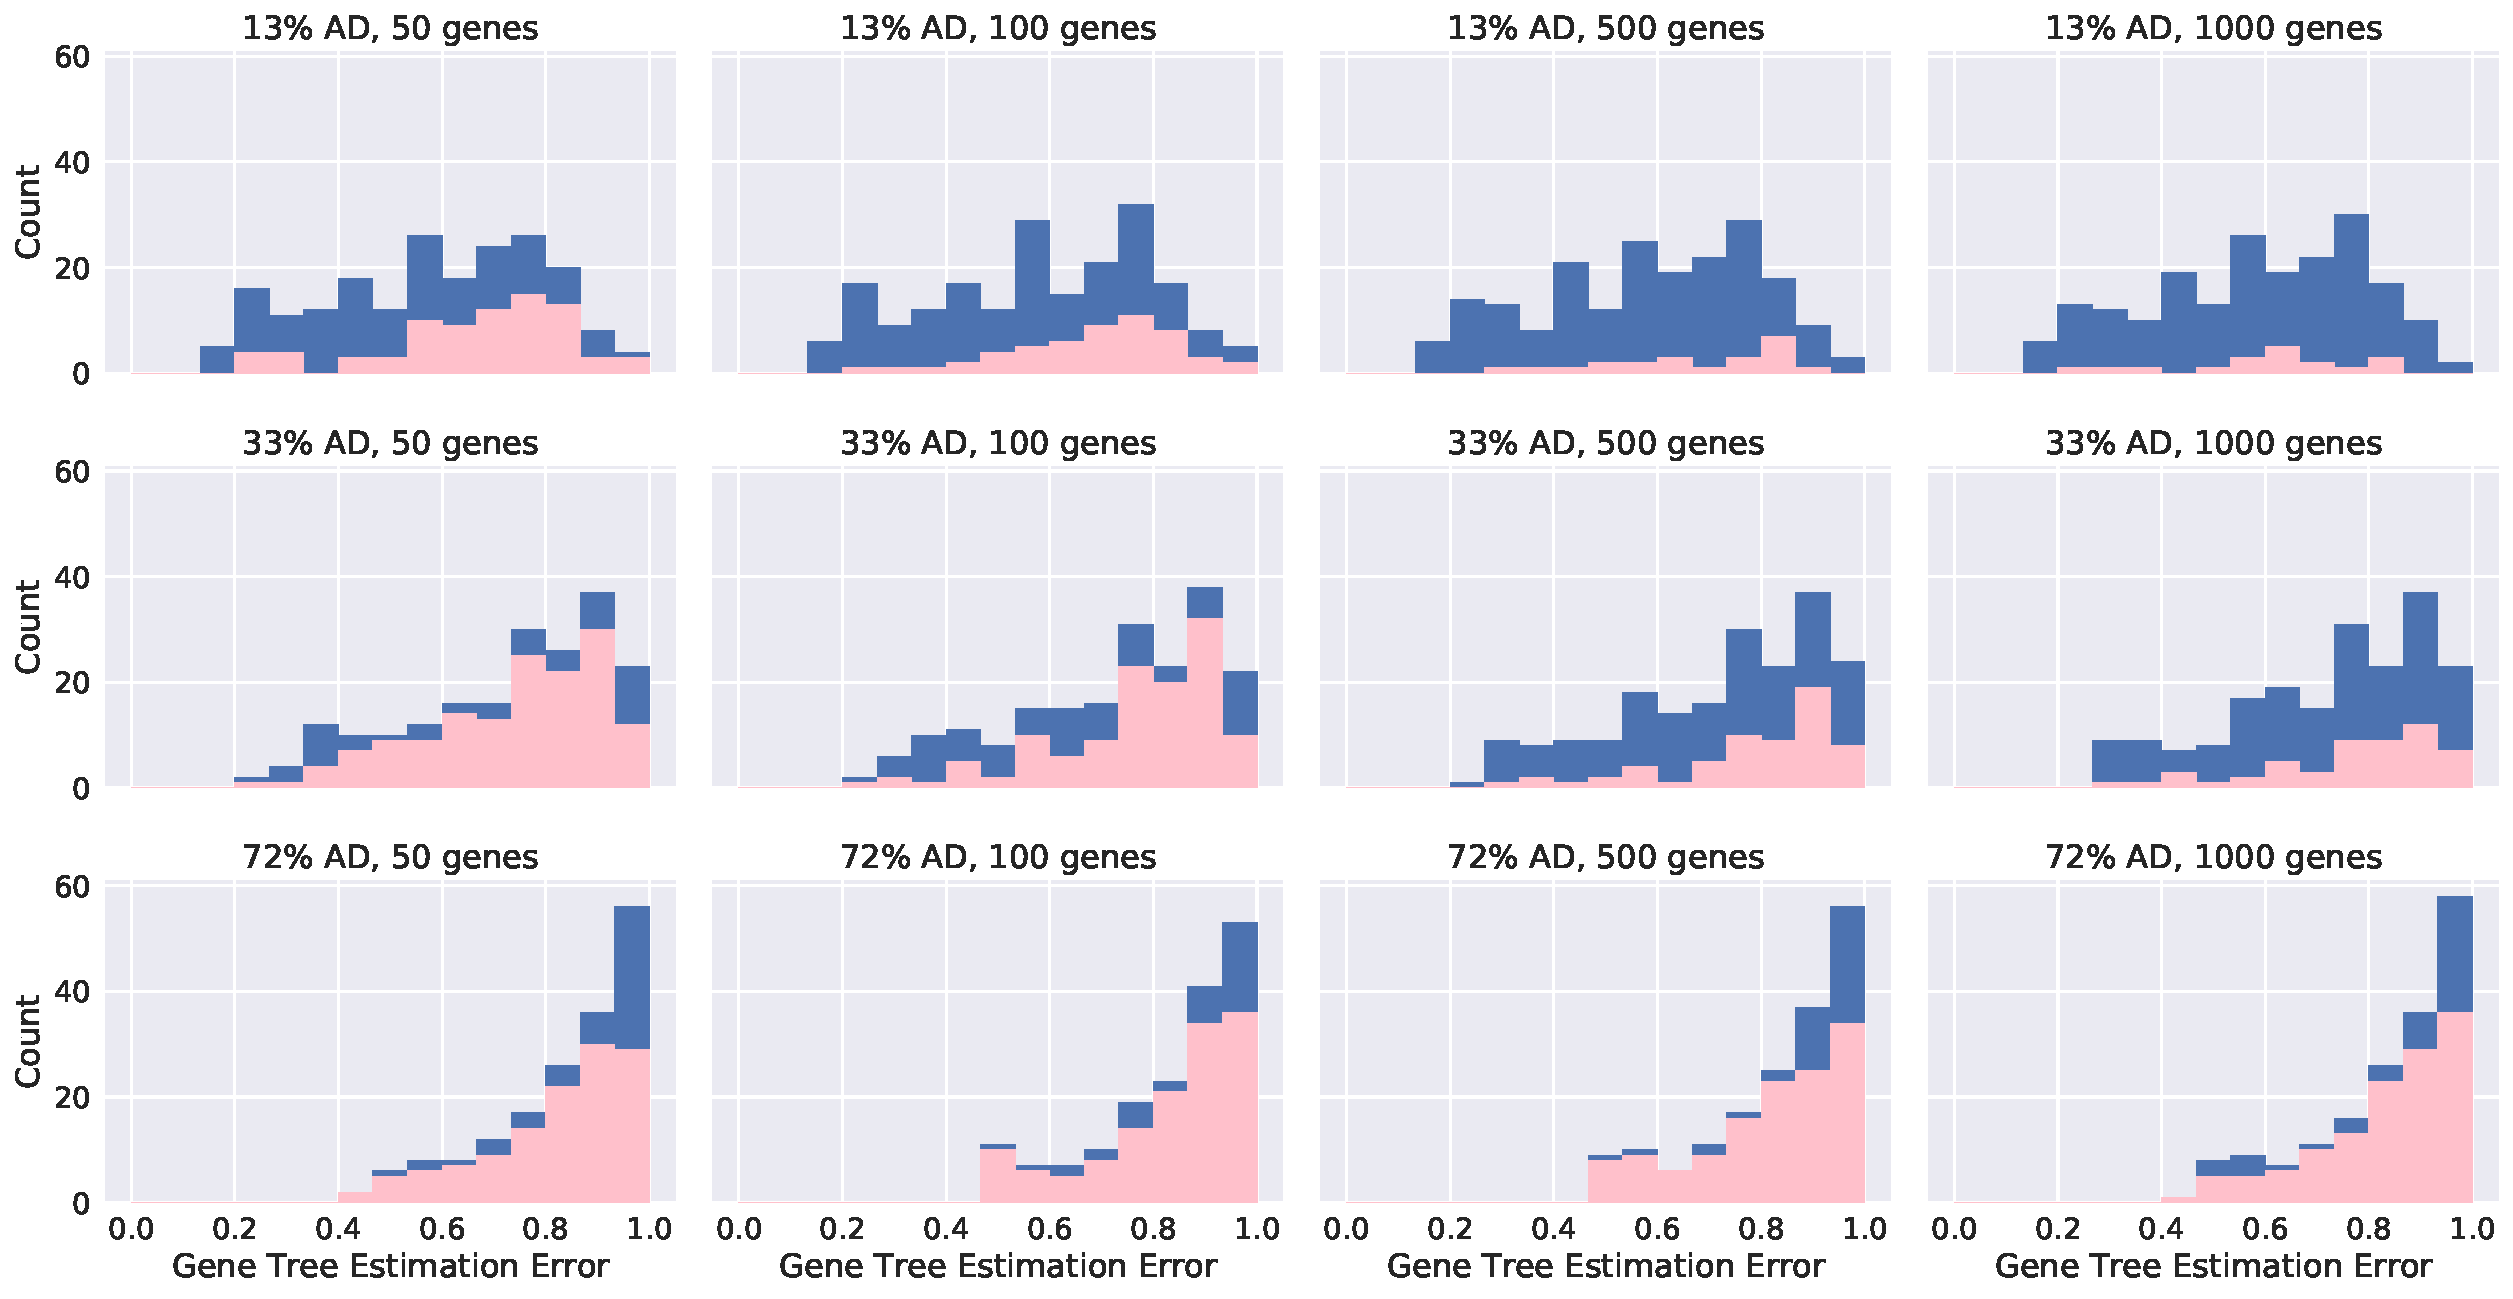
\includegraphics[width=\textwidth]{svdquest-figs/svdquestplus_vs_paup_better_score.pdf}
  \caption[Comparison of SVDquest* and SVDquartets+PAUP* with respect to MQSST scores on 50-taxon simulated data]{Results for Experiment 1 on 50-taxon data, showing how
    often SVDquest* finds better MQSST scores than SVDquartets+PAUP*. Pink
    sections of bars represent replicates where SVDquest* finds a
    better scoring tree; blue sections represent replicates where both
    methods find the same scoring tree. It is impossible for SVDquartets+PAUP* to
    find a better scoring tree than SVDquest*. Total heights of bars
    represent distribution of  gene tree estimation error (maximum possible value is 1.0) in
    datasets. {Each subfigure shows results for 200 replicates, with the exception of the AD=72\% datasets, which have 195-200 replicates each}.}\label{svdquest::fig:exp1_50}

\end{figure}


\begin{figure}
  \centering
  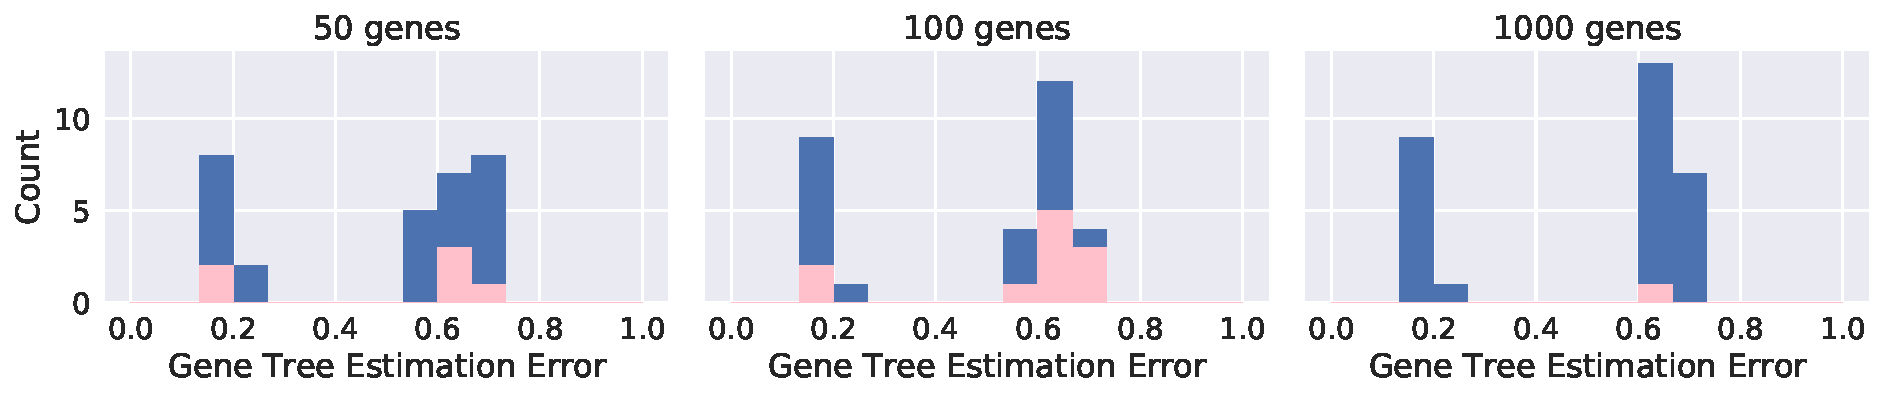
\includegraphics[width=\textwidth]{svdquest-figs/svdquestplus_vs_paup_better_score_15tax.pdf}
  \caption[Comparison of SVDquest* and SVDquartets+PAUP* with respect to MQSST scores on 15-taxon high ILS simulated data]{Results for Experiment 1 on 15-taxon data with 82\% AD
   (high ILS),
    showing how often SVDquest* finds a better scoring tree than
    SVDquartets+PAUP*. Pink sections of bars represent replicates where SVDquest*
    finds a better scoring tree; blue sections represent replicates
    where both methods find the same scoring tree. It is impossible for SVDquartets+PAUP* to
    find a better scoring tree than SVDquest*.  Total heights of
    bars represent distribution of gene tree estimation error (maximum possible value is 1.0) in
    datasets. Each subfigure shows results for 30 replicates.
    }\label{svdquest::fig:exp1_15}
\end{figure}

\begin{figure}
  \centering
  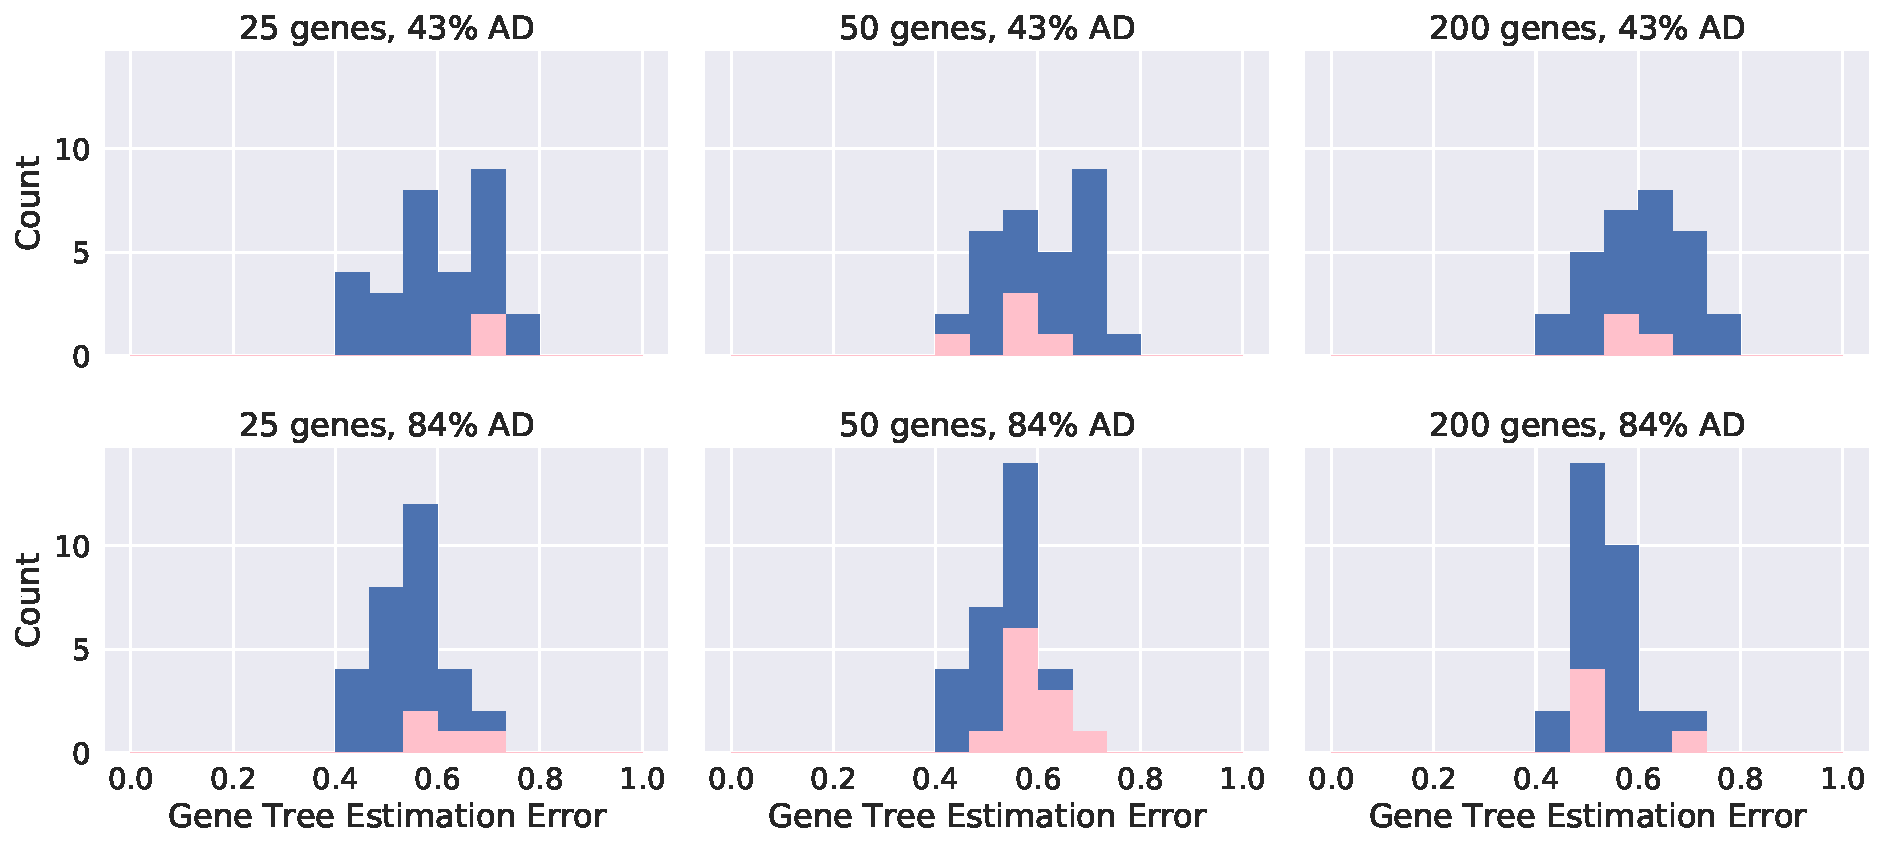
\includegraphics[width=\textwidth]{svdquest-figs/svdquestplus_vs_paup_better_score_10tax.pdf}
\caption[Comparison of SVDquest* and SVDquartets+PAUP* with respect to MQSST scores on 10-taxon simulated data]{Results for Experiment 1 on 10-taxon data, showing how
    often SVDquest* finds a better scoring tree than SVDquartets+PAUP*. Pink
    sections of bars represent replicates where SVDquest* finds a
    better scoring tree; blue sections represent replicates where both
    methods find the same scoring tree. It is impossible for SVDquartets+PAUP* to
    find a better scoring tree than SVDquest*. Total heights of bars
    represent distribution of gene tree estimation error (maximum possible value is 1.0) in the
    datasets.  
      Each subfigure shows results for 30 replicates.   
    }\label{svdquest::fig:exp1_10}
\end{figure}


\clearpage
\subsection{Results for Experiment 2}
%rfdistance

Experiment 2 evaluates  %SVDquest* and 
SVDquest*-strict (i.e., 
the strict consensus of all optimal trees found by SVDquest*, computed using SIESTA) 
in terms of topological accuracy 
on simulated c-gene datasets, and also compares it to ASTRID, ASTRAL, and SVDquartets+PAUP.  
{The comparison between SVDquest*-strict and SVDquartets+PAUP* on the 50-taxon datasets (Figures \ref{fig:s4}-\ref{fig:s7}) shows that although SVDquest*-strict and SVDquartets+PAUP* have similar accuracy, SVDquartets+PAUP* has an advantage over SVDquartets+PAUP*. }

%By varying the level of ILS, GTEE, number of taxa, and number
%of genes, we also see how these dataset properties impact the relative
%and absolute performance of these species tree estimation methods.


%Our first part of this experiment compares  SVDquest*   and SVDquest*-strict.
%%SVDquest* tended to be more accurate than SVDquest (i.e., when it
%%differed from SVDquest, the trees were typically more accurate), suggesting that
%%improving the MQSST scores tended to improve topological accuracy %{(see Supplementary Materials, Figures XX-YY}. 
%Furthermore,  when there was more than one optimal tree, then  the strict consensus %tree of the optimal trees also tended
%to have better  topological accuracy {(see Supplementary Materials, Figures XX-YY)}. 
%Hence, in our remaining comparisons we report accuracy for SVDquest*-strict. 


{A comparison between SVDquest*-strict, ASTRAL, and ASTRID} on the 50-taxon datasets with 500 genes is shown in Figure \ref{svdquest::fig:exp2_50}
({see Figure \ref{fig:s8} for other numbers of genes}).
These datasets do
not evolve under a strict molecular clock and vary in ILS levels
(reflected in AD percentages), GTEE, and number of genes.  ASTRAL and
ASTRID have similar accuracy levels under most conditions.  At low
levels of GTEE, all methods are fairly accurate.  With high GTEE,
SVDquest*-strict is much more accurate than ASTRAL and ASTRID. 
At high levels
of ILS and low GTEE, ASTRAL and ASTRID are more accurate than
SVDquest*-strict.  Across all model conditions, the crossover point where
SVDquest*-strict becomes more accurate is approximately 50\% GTEE. 
SVDquest*-strict
also has a bigger advantage over ASTRAL and ASTRID when ILS levels are
lower and there are more genes. 
In the most extreme case with close to
100\% GTEE, 13\% AD, and 1000 genes
{(see Figure \ref{fig:s8})},
ASTRAL  has approximately 75\% estimation error while
SVDquest*-strict has only 10\% estimation error. 

Figure \ref{svdquest::fig:exp2_15} shows results on the 15-taxon datasets (AD=82\%), which
evolve under a strict molecular clock. 
ASTRAL is the most accurate method in all cases. 
The comparison between SVDquest*-strict and ASTRID shows that SVDquest*-strict
has an advantage for the model conditions with largest number of genes (1000) and highest GTEE (40-60\%),
ASTRID has an advantage for the model conditions with fewest genes (50-100) and lowest GTEE (0-20\%), and
otherwise the two methods have similar species
tree estimation error. 
However, this dataset has a relatively limited
range of gene tree error - no replicate has greater than 60\% average
GTEE, which is the model condition where we would expect the best
performance from SVDquest*-strict. 

Results on the 10-taxon data (which do not evolve under a strict
molecular clock) are shown in Figure \ref{svdquest::fig:exp2_10}.  All three
methods have similar levels of accuracy under most conditions.
However, ASTRAL frequently returns slightly more topologically
accurate trees than the other two methods, and ASTRAL and ASTRID are
somewhat more accurate than SVDquest*-strict when there is low GTEE. Like the
15-taxon data, this model condition has no replicates with greater than
60\% average GTEE.

\clearpage

\begin{figure}
  \centering
  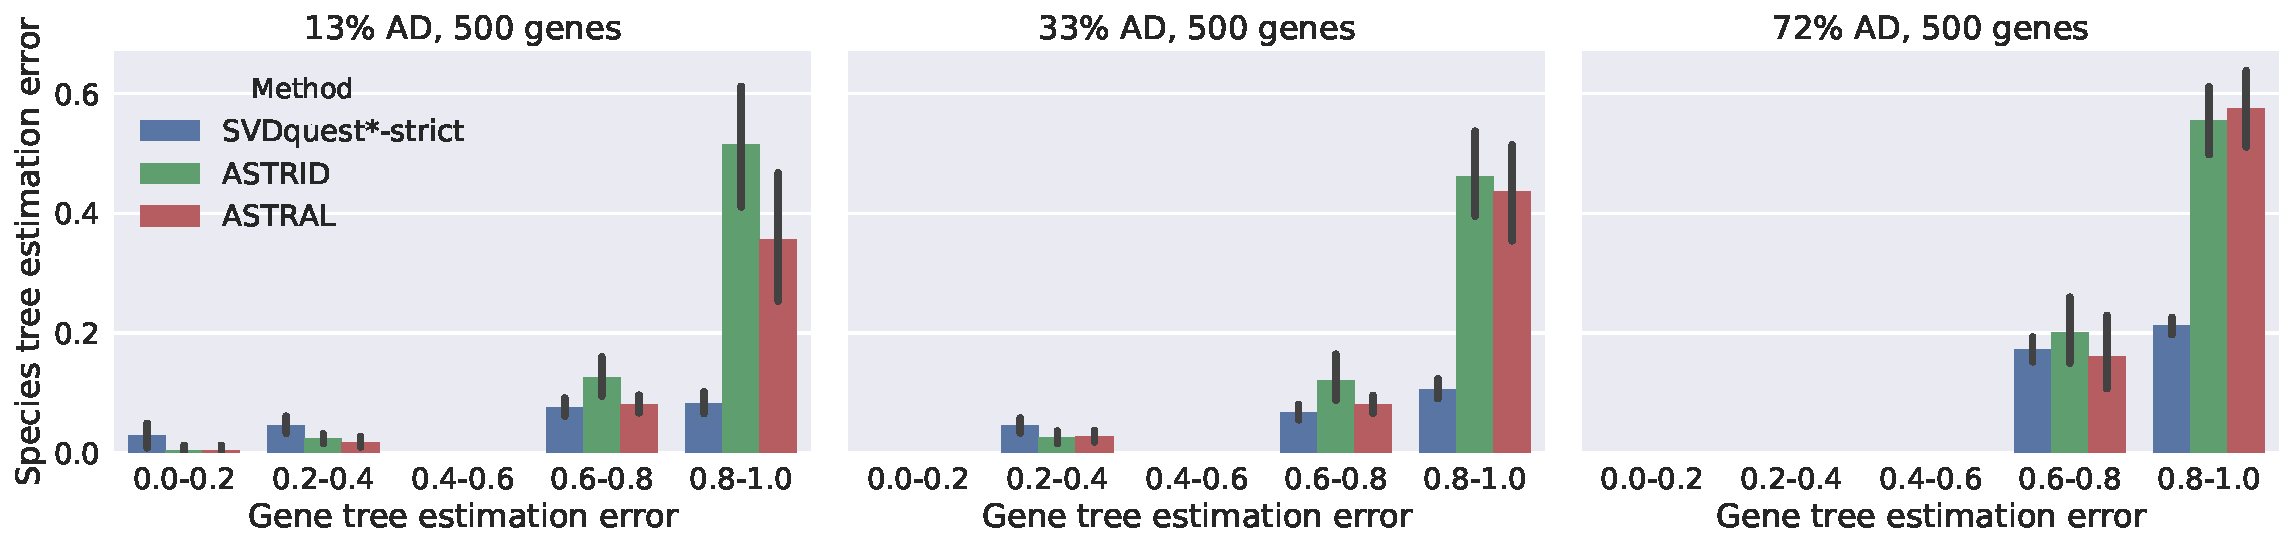
\includegraphics[width=\textwidth]{svdquest-figs/coalescent_rfdists_500.pdf}
  \caption[Species tree topological error rates for 50-taxon simulated data]{Species tree topological error rates (maximum possible is 1.0) for 50-taxon simulated data, as a function of percent
    gene tree estimation error (maximum possible is 1.0); {the first two figures show results for 200 replicates and the last figure shows results for 198 replicates.} 
    Error bars show standard
    error.    
    }\label{svdquest::fig:exp2_50}
    \end{figure}


\begin{figure}
  \centering
  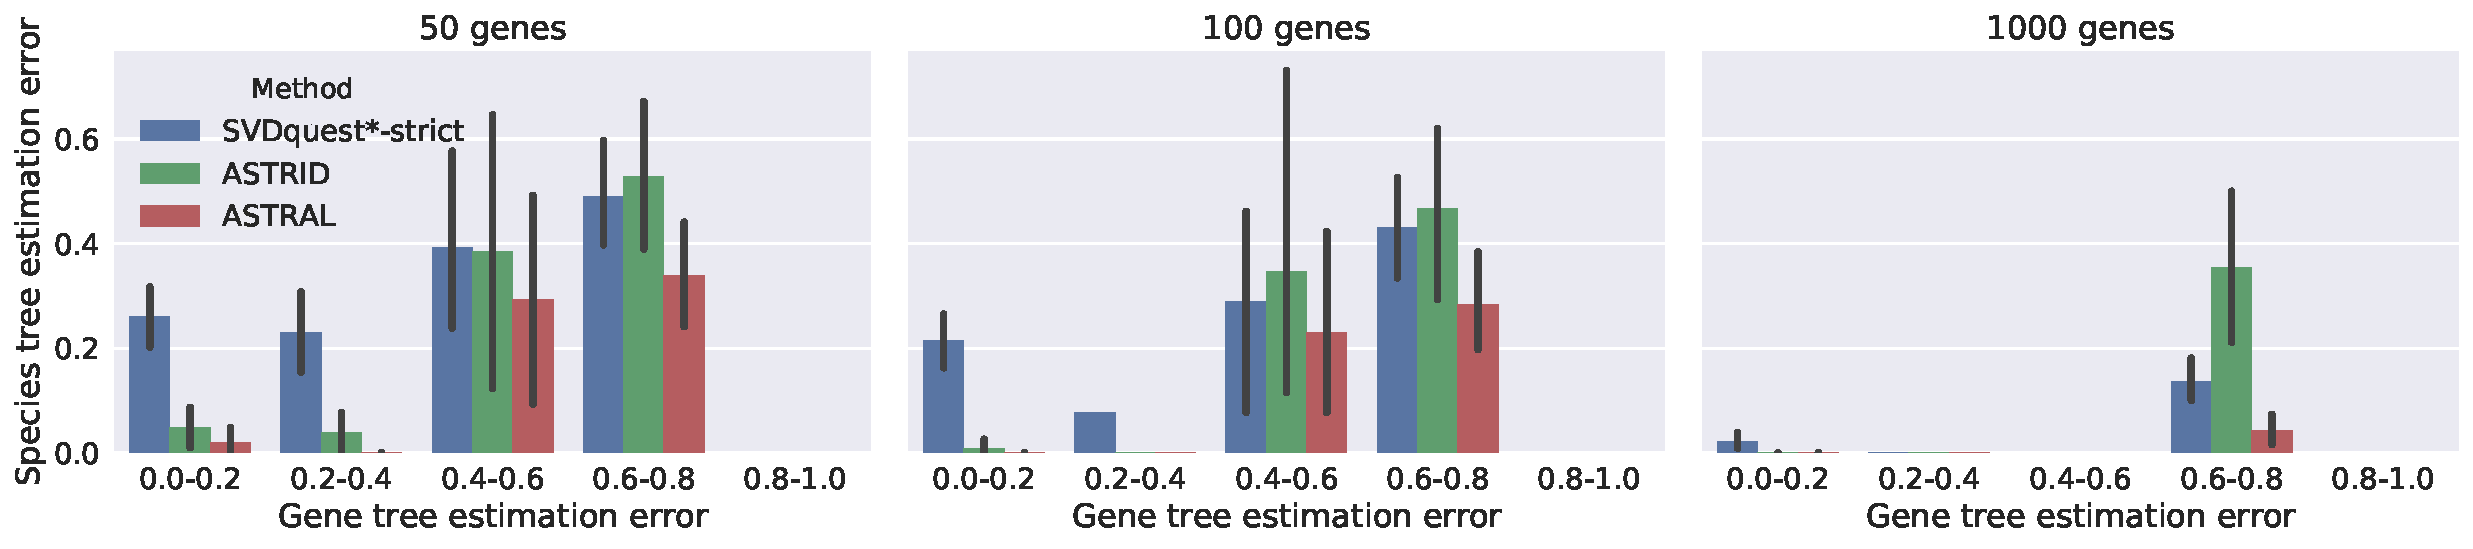
\includegraphics[width=\textwidth]{svdquest-figs/coalescent_rfdists_15tax.pdf}
  \caption[Species tree topological error rates for 15-taxon simulated data]{Species tree topological  error rates (maximum possible is 1.0) 
  for 15-taxon simulated data (AD=82\%), as a
    function of gene tree estimation error (maximum possible is 1.0); each subfigure shows results on 30 replicates. Error bars show standard
    error.   
    }
    \label{svdquest::fig:exp2_15}\end{figure}

\begin{figure}
  \centering
  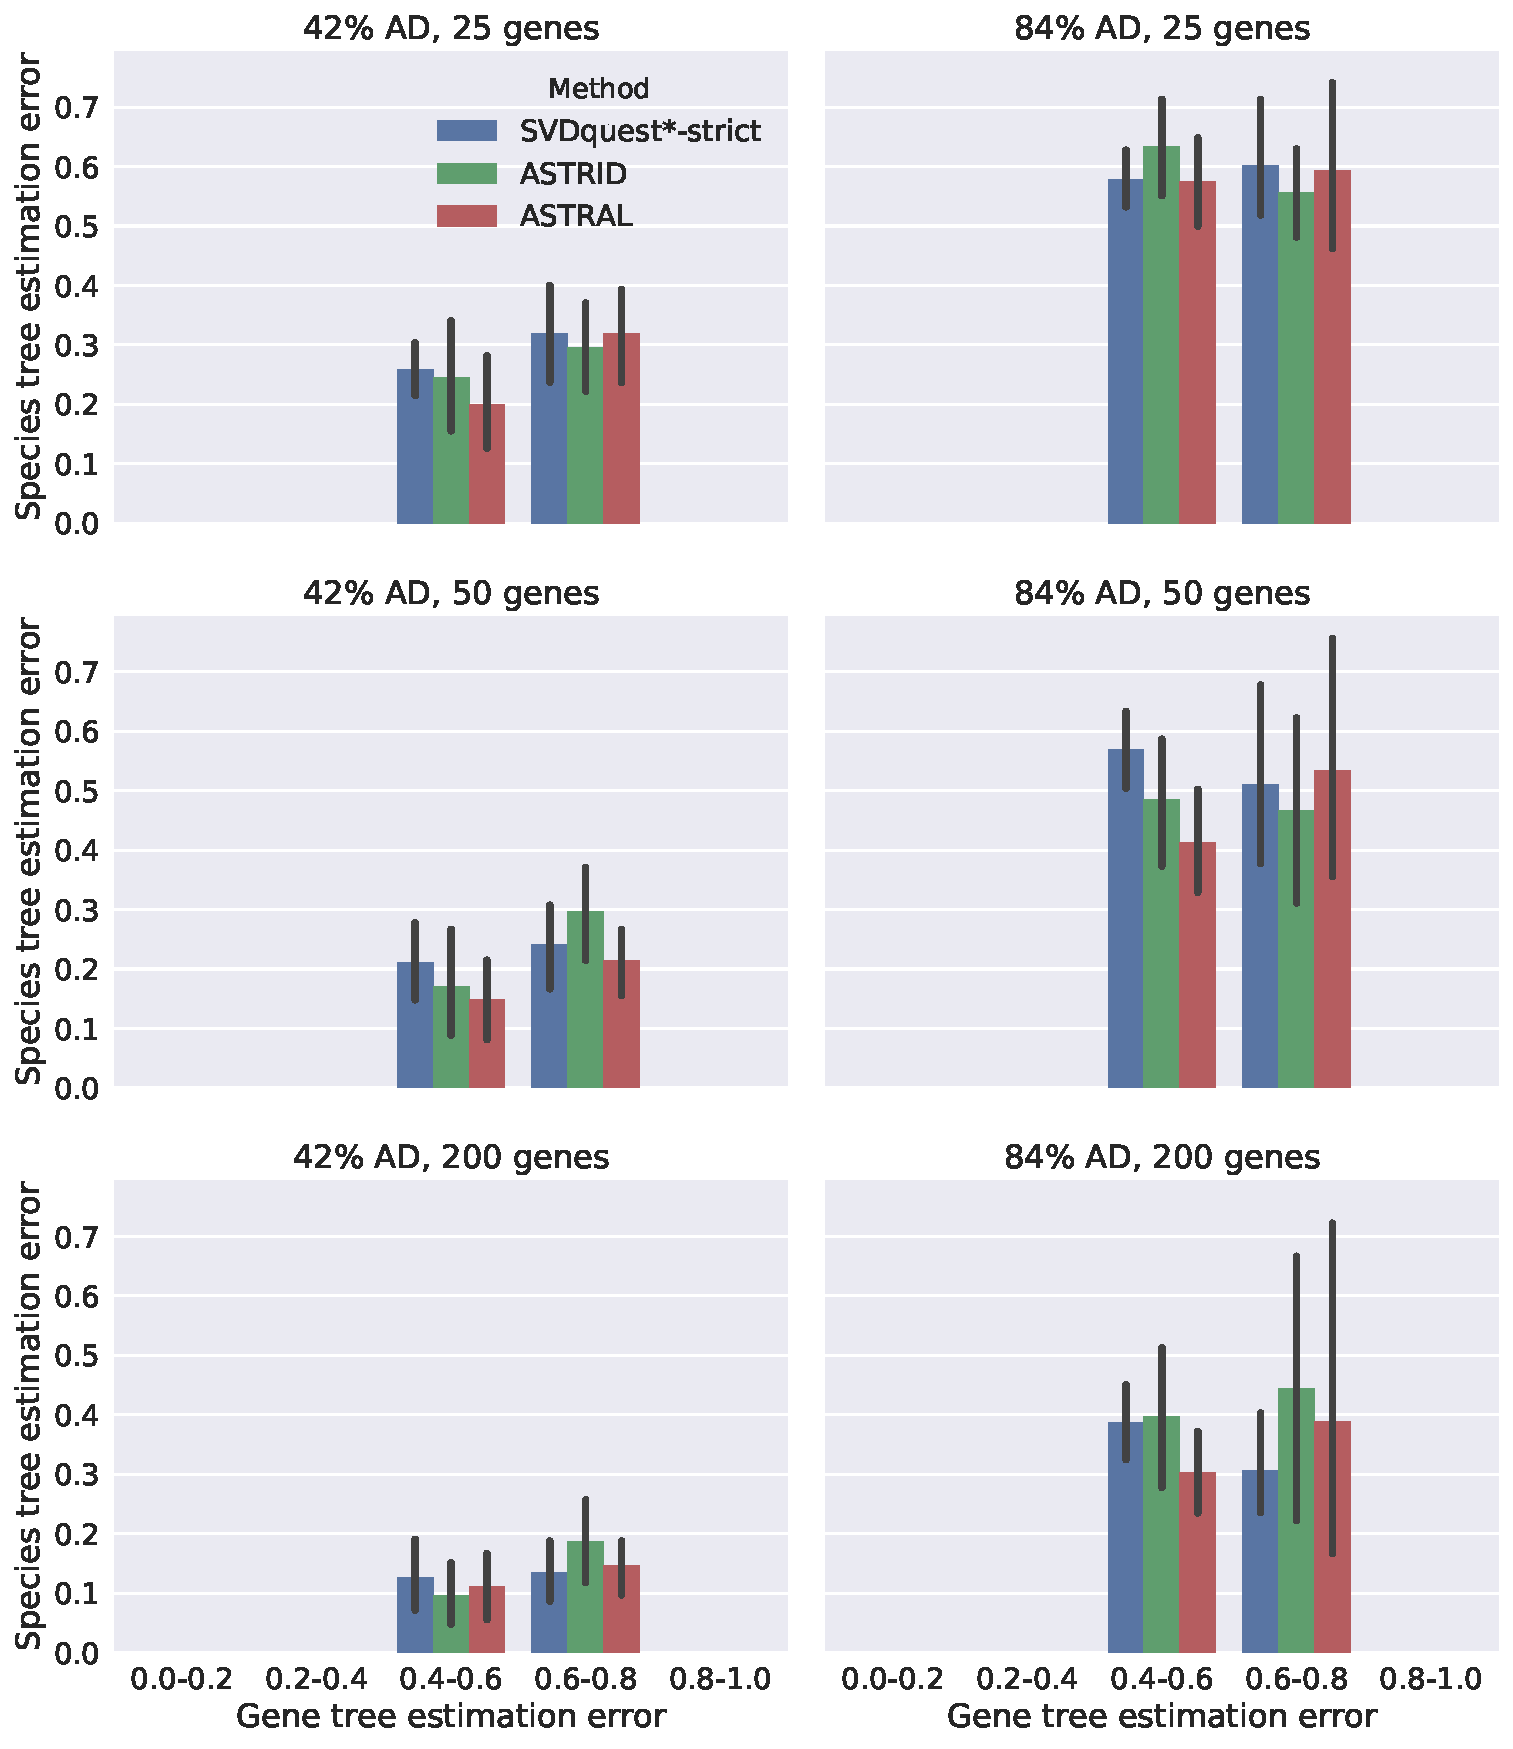
\includegraphics[width=0.8\textwidth]{svdquest-figs/coalescent_rfdists_10tax.pdf}
\caption[Species tree topological error rates for 10-taxon simulated data]{Species tree topological error rates (maximum possible is 1.0) for 10-taxon simulated data, as a
    function of gene tree estimation error (maximum possible is 1.0); each subfigure shows results for 30 replicates. Error bars show standard
    error. 
}
    \label{svdquest::fig:exp2_10}
\end{figure}


\clearpage
\subsection{Results for Experiment 3}

Experiment 3 compares SVDquest*-strict to  ASTRAL, ASTRID, and SVDquartets+PAUP* on supergene datasets (i.e.,  when loci are not
recombination-free). 
We report both MQSST scores and topological accuracy.


The comparison between SVDquartets+PAUP* and SVDquest*-strict shows that
SVDquest*-strict typically matches or improves on SVDquartets+PAUP* with respect to
topological accuracy  {(Figures \ref{fig:s9}-\ref{fig:s11})}. 
In fact, the advantage of using SVDquest*-strict over SVDquartets+PAUP* is greater
on the supergene datasets than on c-gene datasets.
In what follows, we compare SVDquest*-strict to ASTRAL and ASTRID.


Results on the 50-taxon datasets are shown 
in Figure \ref{svdquest::binned_50}. 
The recombination-free loci have only 25 sites; all other
lengths indicate supergenes obtained by combining c-genes.
On all the model
conditions with 25-site loci,
SVDquest*-strict has a substantial advantage over ASTRID and ASTRAL. 
On the
lowest ILS model condition, SVDquest*-strict retains the same accuracy as the
c-genes are combined into supergenes. 
However, as the number of c-genes per supergene increases, ASTRAL and ASTRID become
more accurate,  eventually equaling or improving over SVDquest*-strict. 
For example, on the 33\% AD  model condition, SVDquest*-strict has an
advantage when the supergenes have at most two c-genes, but  then only
ties with ASTRAL and ASTRID when there are 
more c-genes per supergene.  
On the 72\% AD 
model condition, SVDquest*-strict retains an advantage regardless of the
number of c-genes per supergene, but the advantage decreases with the length
of the supergene. 

Results on the 15-taxon datasets are seen in Figure \ref{svdquest::binned_15}.
The c-genes have only 10 sites; all other lengths
indicate supergenes obtained by binning together different c-genes.
At the longest supergenes with 1000 sites (each composed of
100 recombination-free loci), ASTRAL and ASTRID find more accurate
trees than SVDquest*-strict, but at lower levels of binning, SVDquest*-strict finds
trees that are more accurate than ASTRID but less accurate than
ASTRAL. ASTRAL finds slightly more accurate trees when the loci are
recombination-free, while ASTRID improves substantially with increased
binning, especially when there are 1000 loci.  The impact of binning
on SVDquest*-strict is minimal.

Relative performance on the 10-taxon data, shown
in Figure \ref{svdquest::binned_10}, is similar to the
15-taxon data. ASTRAL typically becomes less accurate at higher levels
of binning, while SVDquest*-strict is  relatively unaffected, and ASTRID
sometimes improves. These trends are more evident at the 84\% AD
level; at the 43\% AD level, there is relatively little change with
increased binning.

\clearpage
\begin{figure}
  \centering
  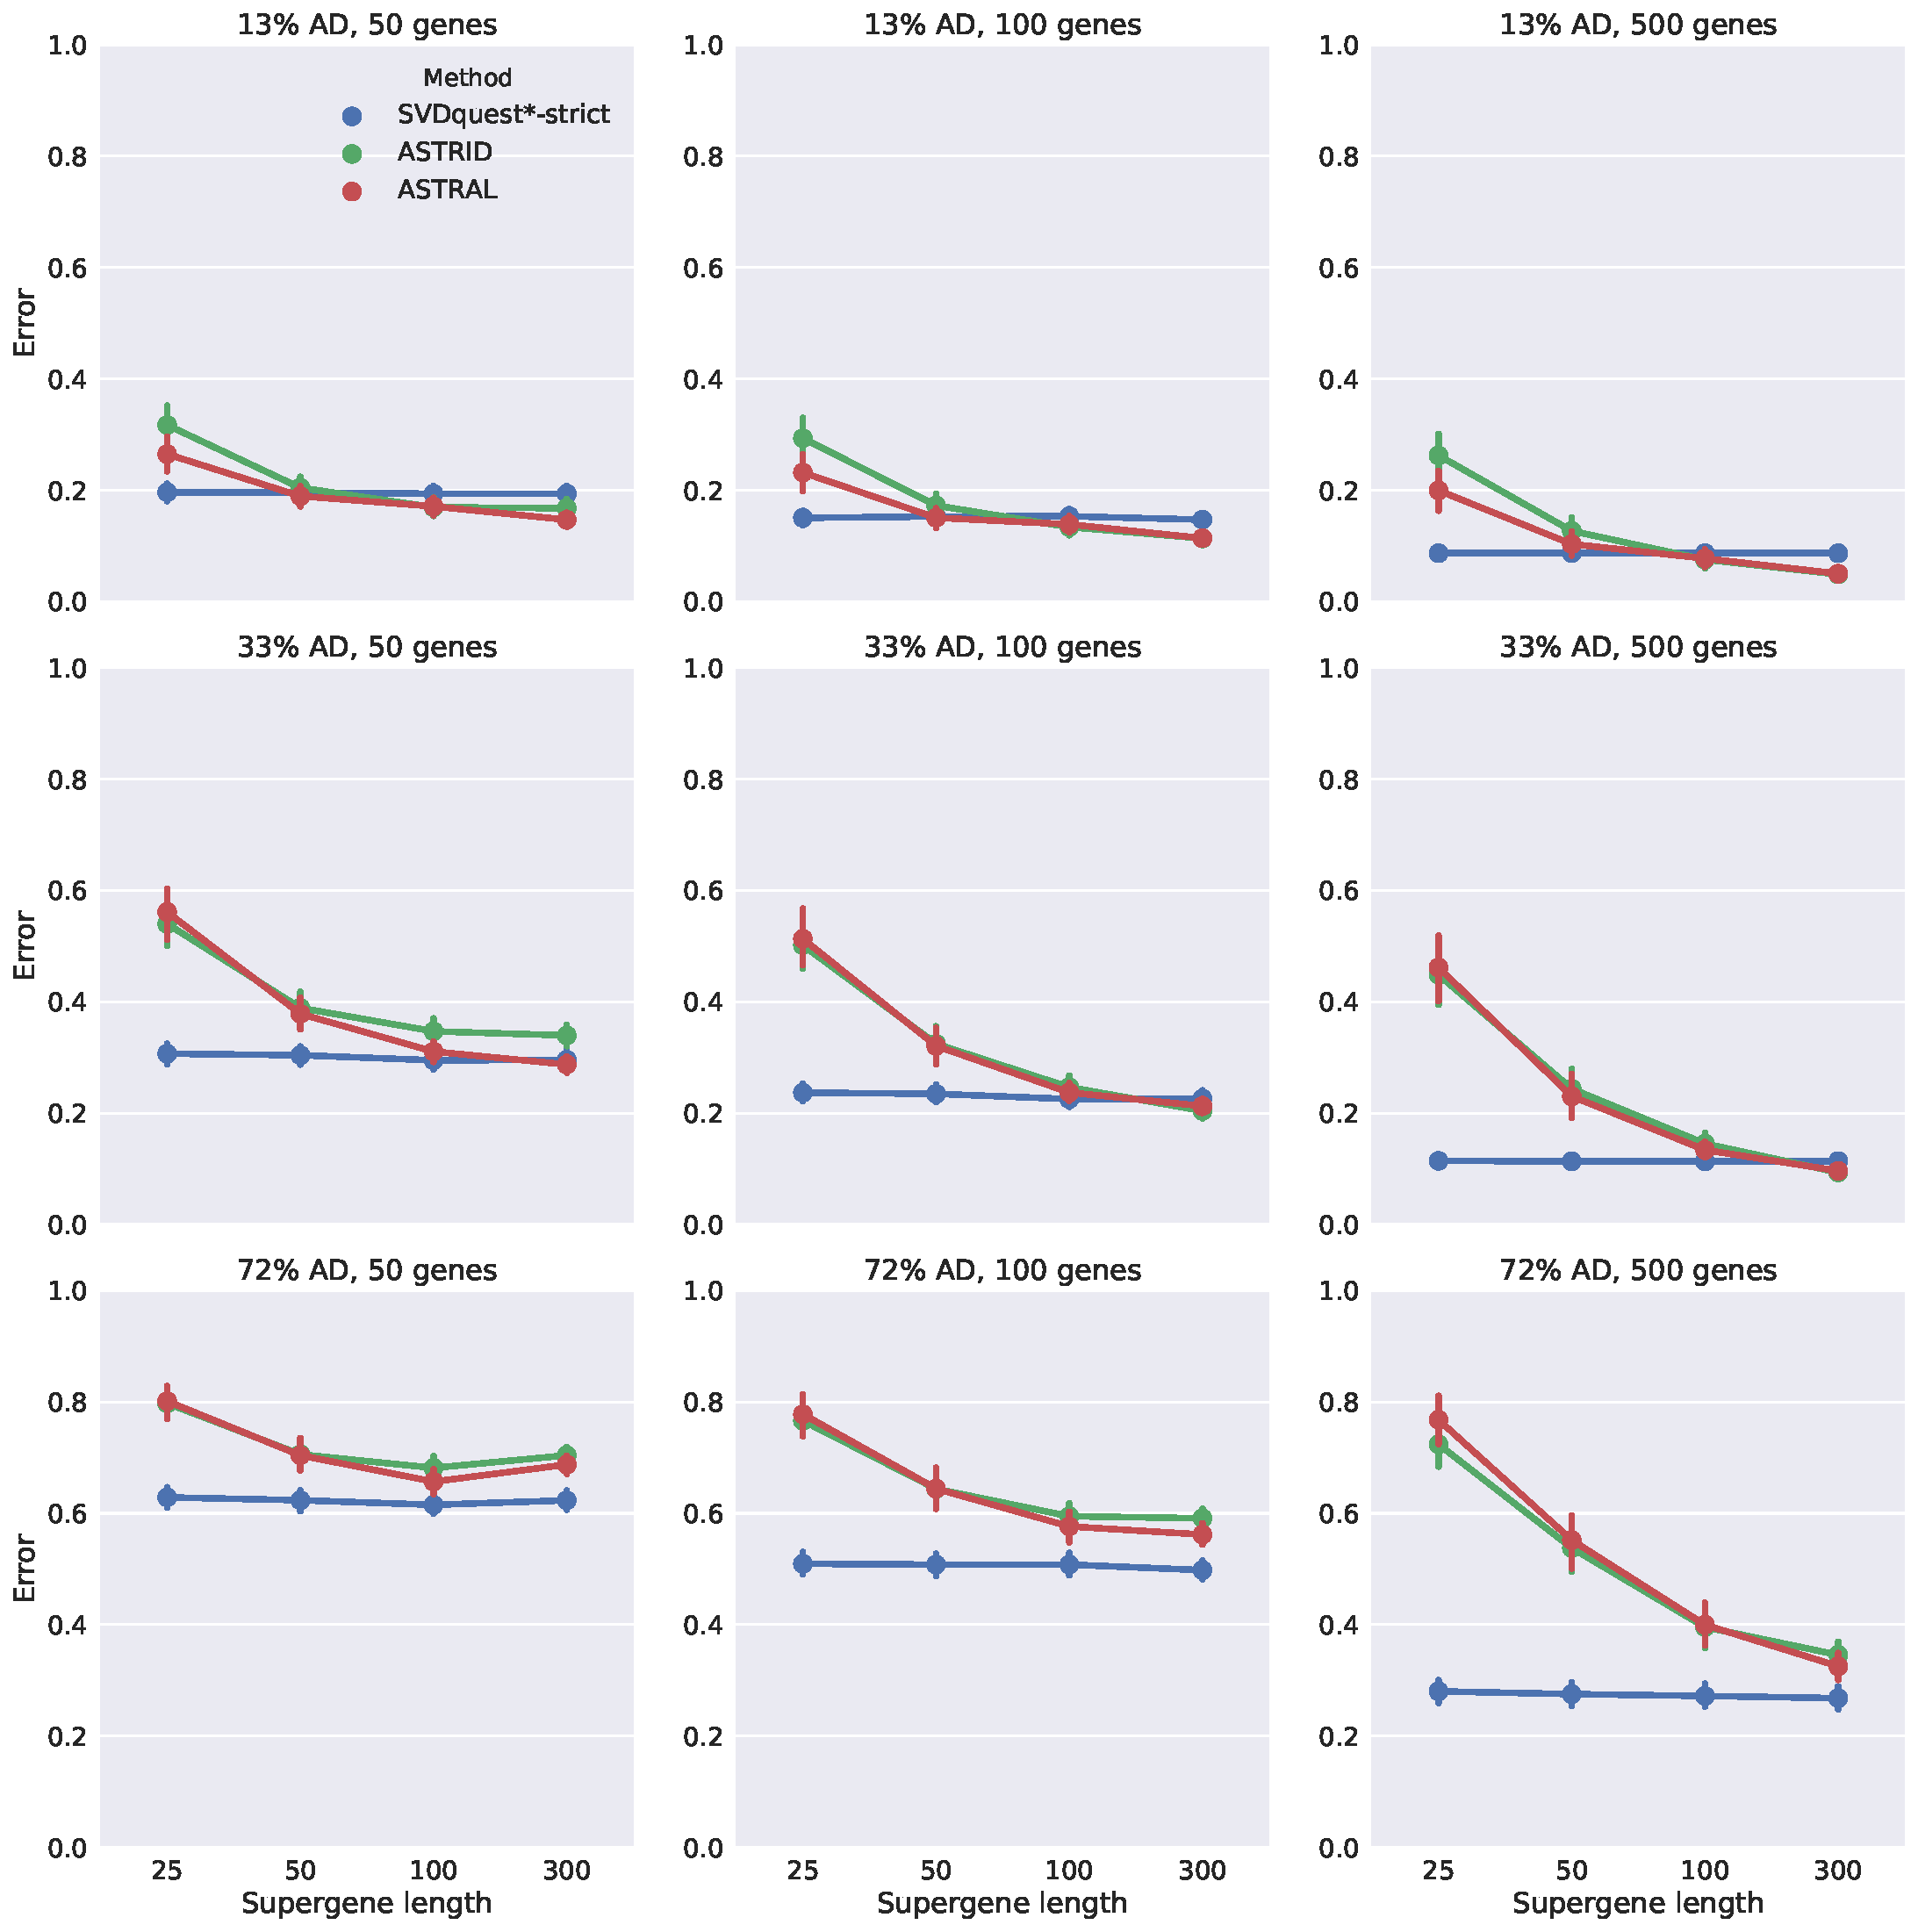
\includegraphics[width=0.9\textwidth]{svdquest-figs/binned_rfdists_nocaml_no1000.pdf}
  \caption[Species tree topological error rates for 50-taxon simulated data with supergenes]{Species tree error rates (maximum possible is 1.0) on 50-taxon simulated data using 
    supergenes (concatenations of c-genes)
    that may not be recombination-free. Error bars represent standard error of the mean. The c-genes in this experiment are 25 sites long, and multiple loci were
    concatenated to form supergenes. Thus, the 
    25-site genes have sites coming from one c-gene, the 50-site genes have
    sites coming from two c-genes, and the 100-site genes have sites coming
    from four c-genes. Each data point in a particular subfigure represents
    an analysis on the same number of sites. 
    {
    Each data point corresponds to an average over 50 replicates, except for the AD=72\% 25-site 50-gene data point, which corresponds to 48 replicates, and 9 other AD=72\%  data points, each of which corresponds to 49 replicates.}
  }\label{svdquest::binned_50}
\end{figure}


\begin{figure}
  \centering
  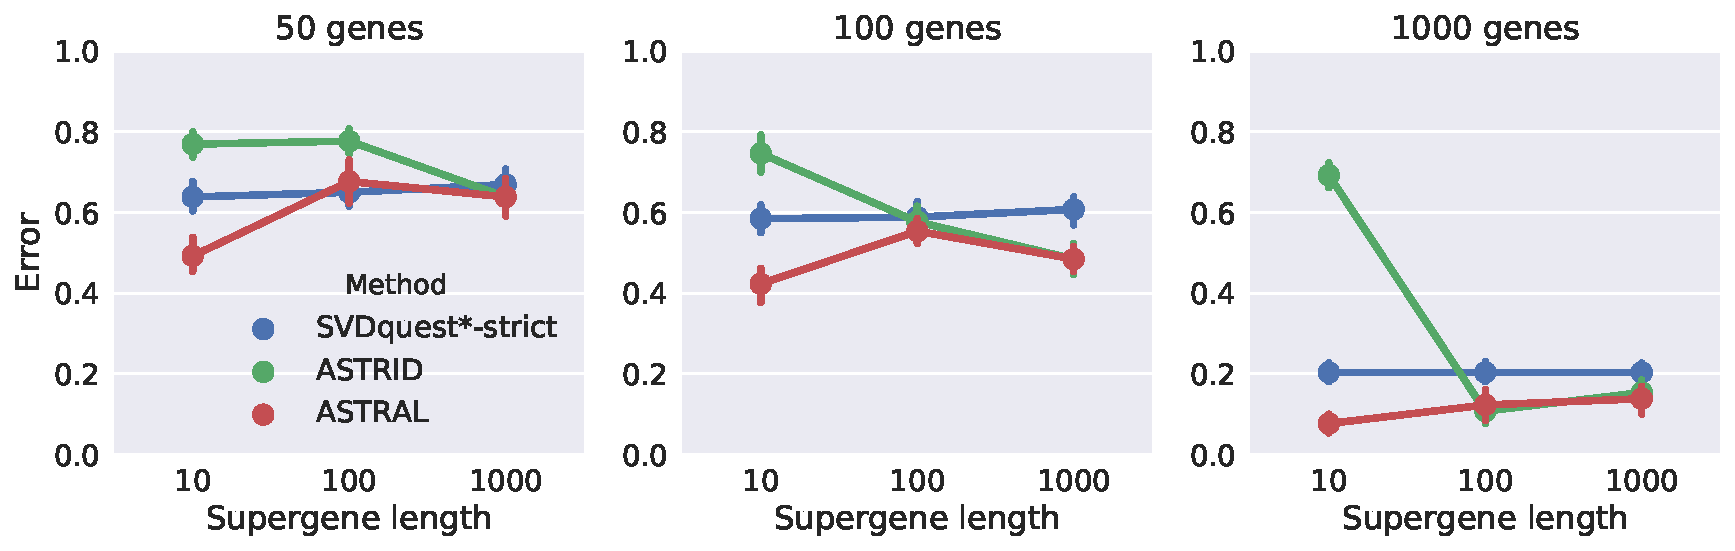
\includegraphics[width=\textwidth]{svdquest-figs/binned_rfdists_nocaml_15tax.pdf}
  \caption[Species tree topological error rates for 15-taxon simulated data with supergenes]{Species tree error rates (maximum possible is 1.0) on 15-taxon simulated data (AD=82\%) for three different numbers of c-genes, then binned into 
    supergenes (concatenations of c-genes); results shown are averaged over 10 replicates with error bars
    representing standard error of the mean.
    The c-genes in this experiment
    have 10 sites, so that longer loci are supergenes.  Each data point in a particular
    subfigure represents an analysis on the same total number of sites. 
    }\label{svdquest::binned_15}
\end{figure}



\begin{figure}
  \centering
  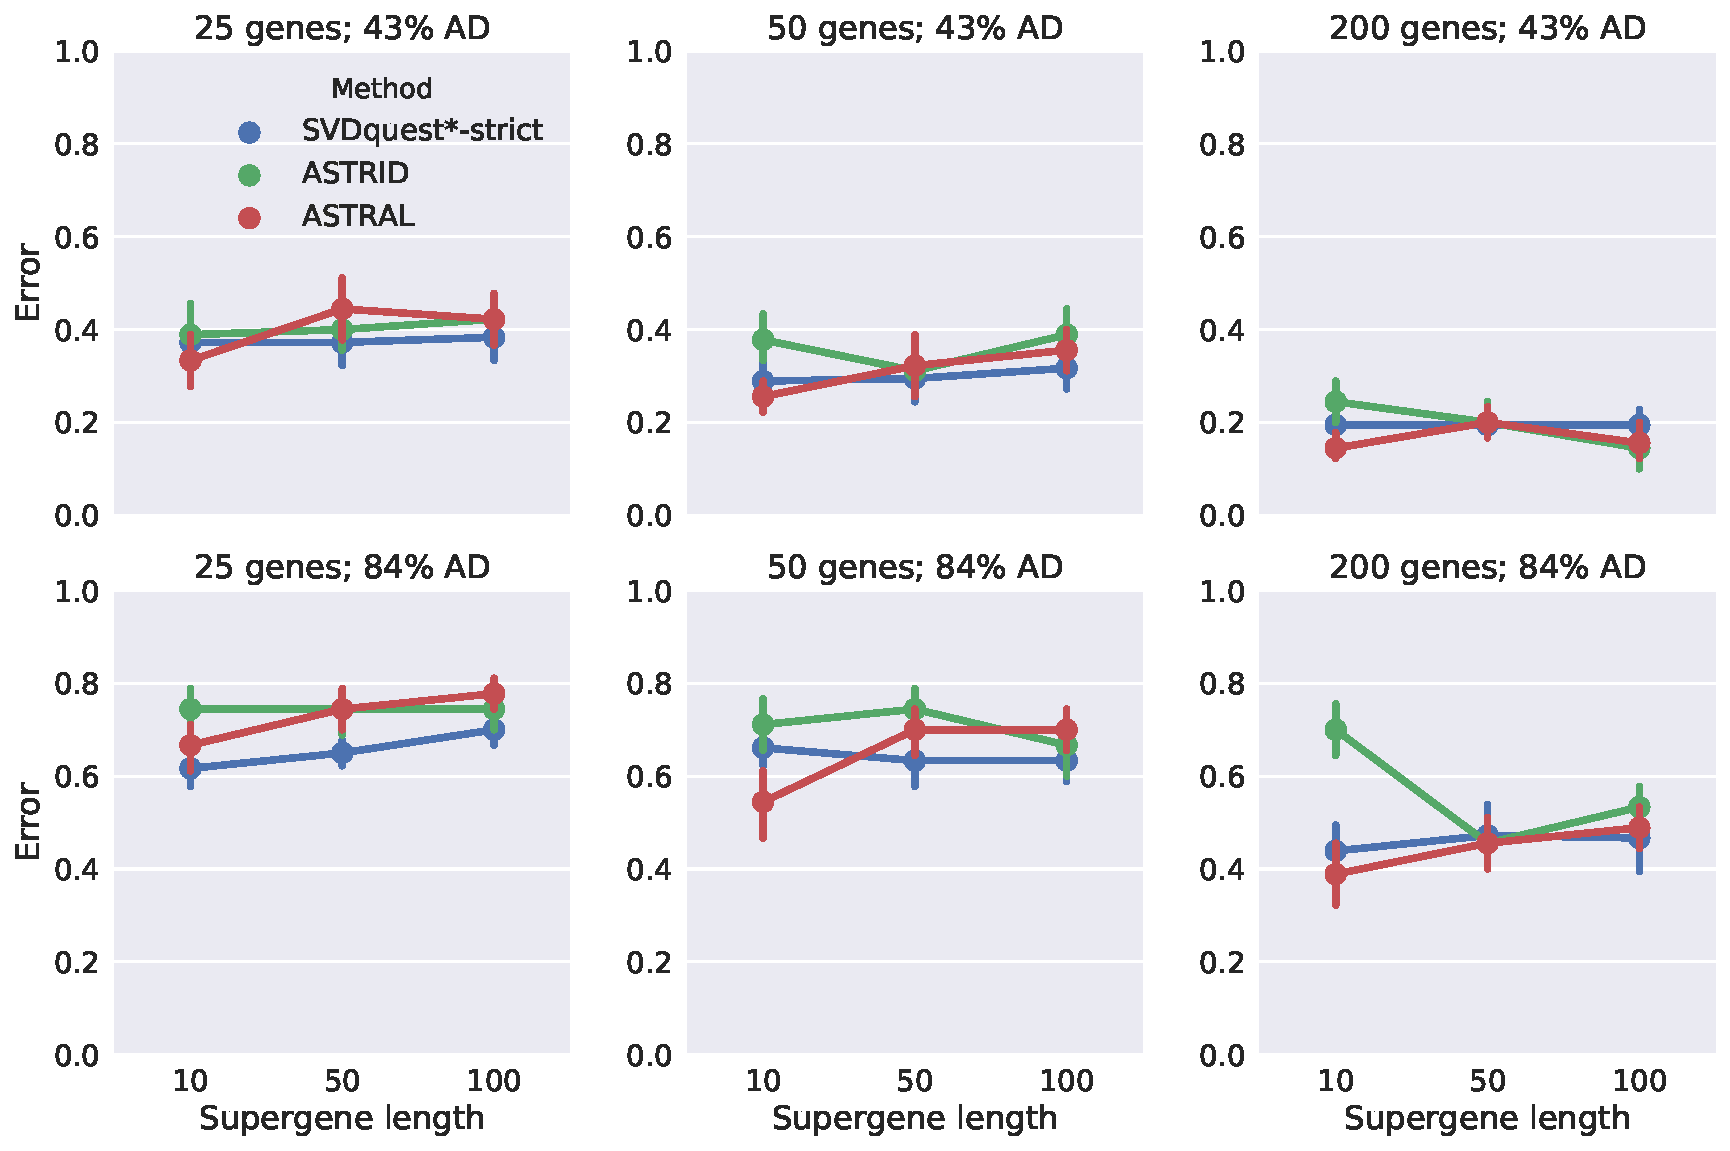
\includegraphics[width=\textwidth]{svdquest-figs/binned_rfdists_nocaml_10tax.pdf}
  \caption[Species tree topological error rates for 10-taxon simulated data with supergenes]{Species tree error rates (maximum possible is 1.0) on 10-taxon simulated data using
    supergenes (concatenations of c-genes), averaged over 10 replicates; error bars
    represent standard error of the mean. The c-genes in this experiment
    have 10 sites, and longer sequences are supergenes.
    Each data point in a particular subfigure
    represents an analysis on the same number of sites. 
    }\label{svdquest::binned_10}
\end{figure}


\clearpage

\subsection{Results for Experiment 4}

Experiment 4 compares coalescent-based methods to unpartitioned
concatenation using RAxML (i.e., CA-ML) on simulated datasets.  On the 50-taxon data, seen in
Figure \ref{svdquest::fig:exp3_50} for 500 gene datasets
{(see Figure \ref{fig:s8} for other numbers of genes)},
CA-ML and SVDquest*-strict tend to perform similarly, and better than ASTRID
and ASTRAL when GTEE is greater than 60\%.  
On the lower ILS (13\% AD)
condition, CA-ML is somewhat more accurate than SVDquest*-strict when there
are fewer genes  {(Figure \ref{fig:s8})}, but this advantage is
reduced for 500 or 1000 genes. At the highest ILS level, CA-ML is
actually less accurate than SVDquest*-strict when there are few genes and low
GTEE, but both of these methods are less accurate than ASTRAL and
ASTRID.

On the 15-taxon data (AD=82\%), shown in Figure \ref{svdquest::fig:exp3_15}, 
ASTRAL is always the
most accurate method. ASTRID performs worse than CA-ML and
SVDquest*-strict when there are 50 or 100 genes. With 1000 genes, all methods
perform well, but ASTRAL and ASTRID slightly outperform CA-ML and
SVDquest*-strict. 

On the 10-taxon data, shown in Figure \ref{svdquest::fig:exp3_10}, CA-ML is
typically the best method on the 43\% AD  data. 
CA-ML slightly
outperforms the other methods except when there are 50 genes and low
GTEE, in which case ASTRAL and ASTRID perform slightly better. On the
84\% AD  data, SVDquest*-strict and CA-ML are the worst performing
methods, and ASTRAL is typically the best method.

We calculated the rank correlation coefficient between
the MQSST scores and topological errors for PAUP* and SVDquest* in
order to determine whether a better MQSST score was correlated with a topologically
more accurate tree. 
We found that there was a statistically
significant correlation ($P < 0.05$) with a Spearman rank correlation coefficient of $\rho = 0.32$ for the 50-taxon datasets.


\subsubsection{Results for Experiment 5}



We compared SVDquest* to  SVDquartets+PAUP*, CA-ML, ASTRAL, and ASTRID trees
on the mammalian biological dataset.
CA-ML, ASTRAL, and ASTRID all return the same tree, 
which recovers the major accepted mammalian clades and
the relationships between them, but SVDquest* 
 {returns a  single tree that is different from the tree found
 by the other methods.}
 {See Figure \ref{svdquest::fig:mammalian-svdquestplus} for the SVDquest* tree with bootstrap branch support, and Figure \ref{fig:s12} for the ASTRAL/ASTRID/CA-ML tree with ASTRAL branch support. }
 The SVDquest* tree has very high bootstrap branch support on
nearly all the edges (100\% support on all but four edges and 99\% support on one edge), and the ASTRAL/CA-ML/ASTRID tree has over 90\% support using ASTRAL's local posterior probability for all of its branches.


 

The SVDquest* tree  agrees with SVDquartets+PAUP*  but differs from
the tree found using CA-ML, ASTRID, and ASTRID in two ways: the placement of tree shrews
(Scandentia) and the topology of the clade Scrotifera with respect to
the placement of bats (Chiroptera).
CA-ML, ASTRAL and ASTRID place
Scandentia as sister to Glires, while SVDquest* places Scandentia as
sister to Primates. 
Both these placements have 100\% support 
(bootstrap support for the SVDquest* tree,
local support for the ASTRAL/CA-ML/ASTRID tree). 
%In addition, the ASTRAL/CA-ML/ASTRID tree has over 90\% support using ASTRAL's local posterior probability for all of its branches. 


Scrotifera consists of three major clades - Chiroptera (bats),
Cetartiodactyla (even-toed ungulates and cetaceans), and Zooamata
(odd-toed ungulates and carnivores). 
CA-ML, ASTRAL and ASTRID resolve
this clade with Chiroptera as the outgroup with 90\% local
support. SVDquest* resolves this with Zooamata as the outgroup, but
with very low support (only 23\% bootstrap support using the modified bootstrapping technique).

The existing literature presents varied hypotheses for Scrotifera. The
SVDquest* analysis presents support for a clade that consists of
Cetartiodactyla and Chiroptera, which has been presented by
\cite{hou2009phylogeny}. 
The CA-ML, ASTRAL, and ASTRID analyses
present support for Fereuungulata, which contains Cetartiodactyla and
Zooamata. 
More recent analyses \cite{zhou2012phylogenomic} have found
increased support for Fereuungulata over Cetartiodactyla+Chiroptera,
but the phylogeny is not yet settled.  However, the bootstrap support
for Cetartiodactyla+Chiroptera in the SVDquest* tree is quite low
(only 23\%), and collapsing this edge makes the tree compatible with
both of these two possibilities.  
SVDquest* establishes
Zooamata with 69\% support, which is only moderate. Collapsing
edges in the SVDquest* tree with less than 75\% bootstrap support 
resolves Cetartiodactyla,
Chiroptera, Carnivora, and Perissodactyla as clades, but does not
determine a relationship between them.


Finally, we also performed the standard non-parametric bootstrapping analysis on
the SVDquest* tree, to evaluate the impact of using the modified bootstrapping technique for defining branch support.
The results from the two techniques were nearly identical. 
All but three of the branches in the SVDquest* tree received exactly the same
support using both techniques (91\% for one branch, 100\% for all the others). 
The differences in the support for the remaining three branches were very small.
One branch that had  99\% using the modified technique had 100\% using the
standard technique.
The  remaining two branches had support less than 75\% using the modified 
bootstrapping technique, and their support changed by at most 5\%: 
Ceteratiodactyla+Chiroptera received  branch support of 23\% using the modified
technique and 19\% using the standard technique, 
Zoomata received 69\% support using the modified technique and 74\% using 
the standard technique. 
Thus, the  modified bootstrapping technique to provide branch support
produces branch support values that are very close to that produced using
the standard bootstrapping technique, while being much faster.


\subsubsection{Experiment 6: Running Time}
We compare the (sequential) running times of ASTRAL,  SVDquest*, and SVDquartets+PAUP* 
on the 37-species mammalian dataset with 424 loci and a total of 1,338,678 characters.  
SVDquartets+PAUP* completed in under 4 minutes. 
ASTRAL and ASTRID both finished in just under 3.5 hours (less than one second difference),   of which all but 4 seconds was spent computing ML gene trees. 
%ASTRID finished in just over 3 hours and 30 minutes, where computing the gene trees took all but 0.25 seconds.
SVDquest*  returned only one tree, and 
completed in under 3 hours and 32 minutes, which was just seconds more than what was needed to compute the ASTRAL and SVDquartets+PAUP* trees.
The detailed running time analysis for SVDquest* is as follows:
\begin{itemize}
\item
Computing maximum likelihood gene trees: 210 minutes
\item
Applying ASTRAL to the set of maximum likelihood gene trees, to obtain the constraint set of bipartitions: 6 seconds.
\item 
Using PAUP* to compute SVDquartets  quartet weights: 3 minutes.   
\item
Applying  PAUP* to the quartet trees to return the species tree:  $<$ 1 second.
\item
Running the dynamic programming within SVDquest* to find   the optimal tree: 1 second.
\end{itemize}
%The total time is just under 184 minutes, but 180 minutes of this is spent computing
%%the maximum likelihood gene trees. 
%Constraint set: 5.7s
%_ Quartet weights: 179.9s
%_ Find tripartition weights: 1.0s
%_ Find optimal trees/SIESTA: 0.009s
%In contrast,  SVDquartets+PAUP*  completes in at most 4 minutes.
Thus,  the running time for SVDquest* (and for SVDquest*-strict) is essentially no different from that of running ASTRAL or ASTRID, and is dominated by the time used to compute ML gene trees. 
Also, SVDquartets+PAUP* is much faster than SVDquest*  because SVDquartets+PAUP* does not need to compute gene trees. 


\clearpage

\begin{figure}
  \centering
  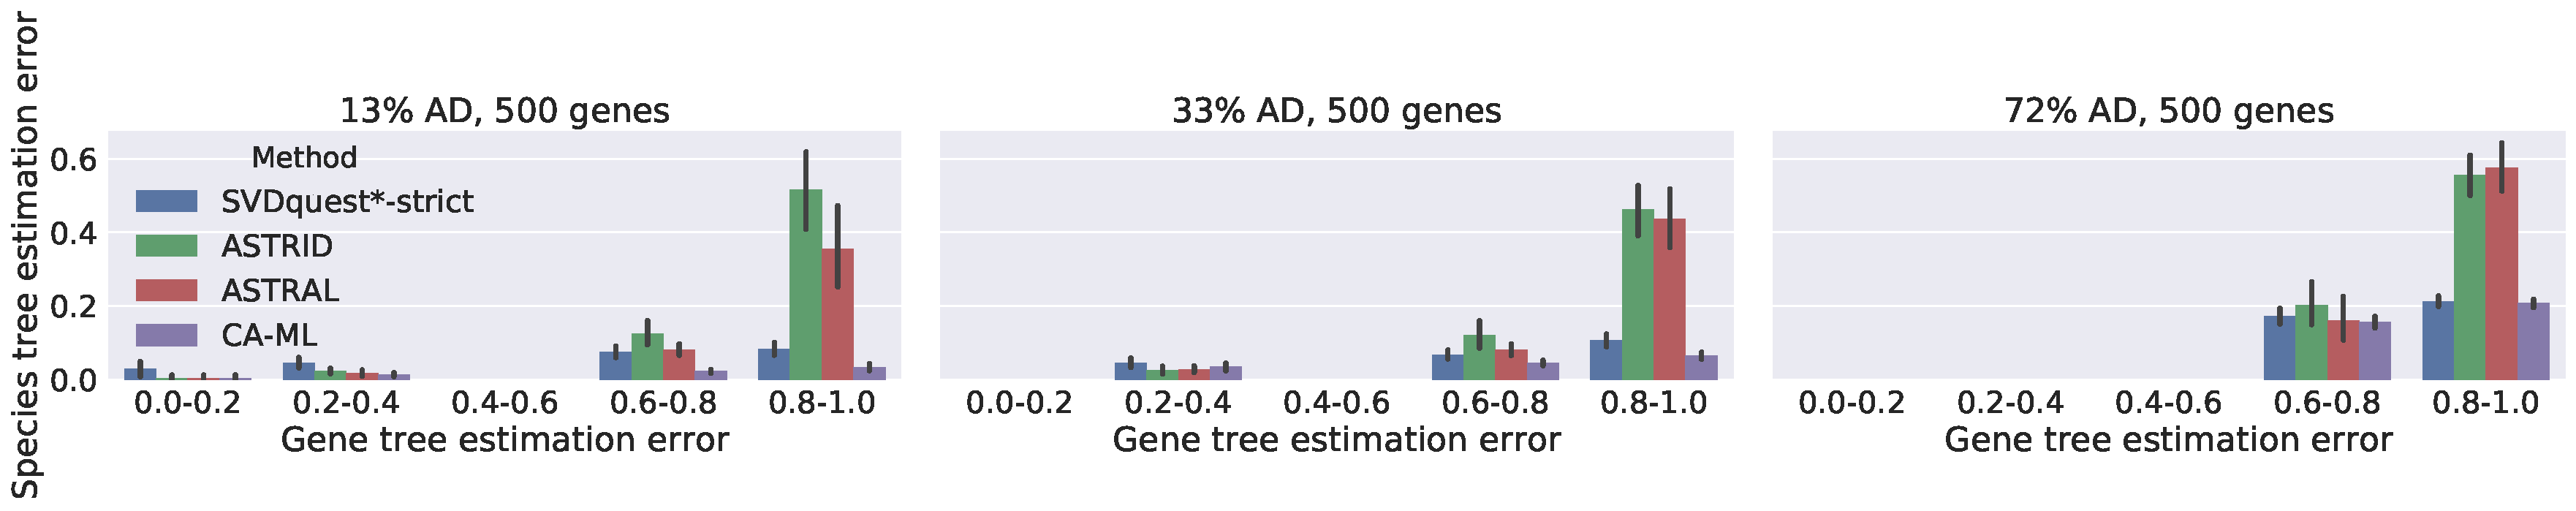
\includegraphics[width=\textwidth]{svdquest-figs/concat_rfdists_500.pdf}
\caption[Species tree topological error rates for 50-taxon simulated data as a function of gene tree estimation error]{Species tree topological error rates (maximum possible is 1.0) for 50-taxon simulated data, as a function of
    gene tree estimation error (maximum possible is 1.0).
    {Each figure shows means and standard
    error; results in the first two subfigures are for 200 replicates  and 198 replicates for the third subfigure.} }
\label{svdquest::fig:exp3_50}\end{figure}


\begin{figure}
  \centering
  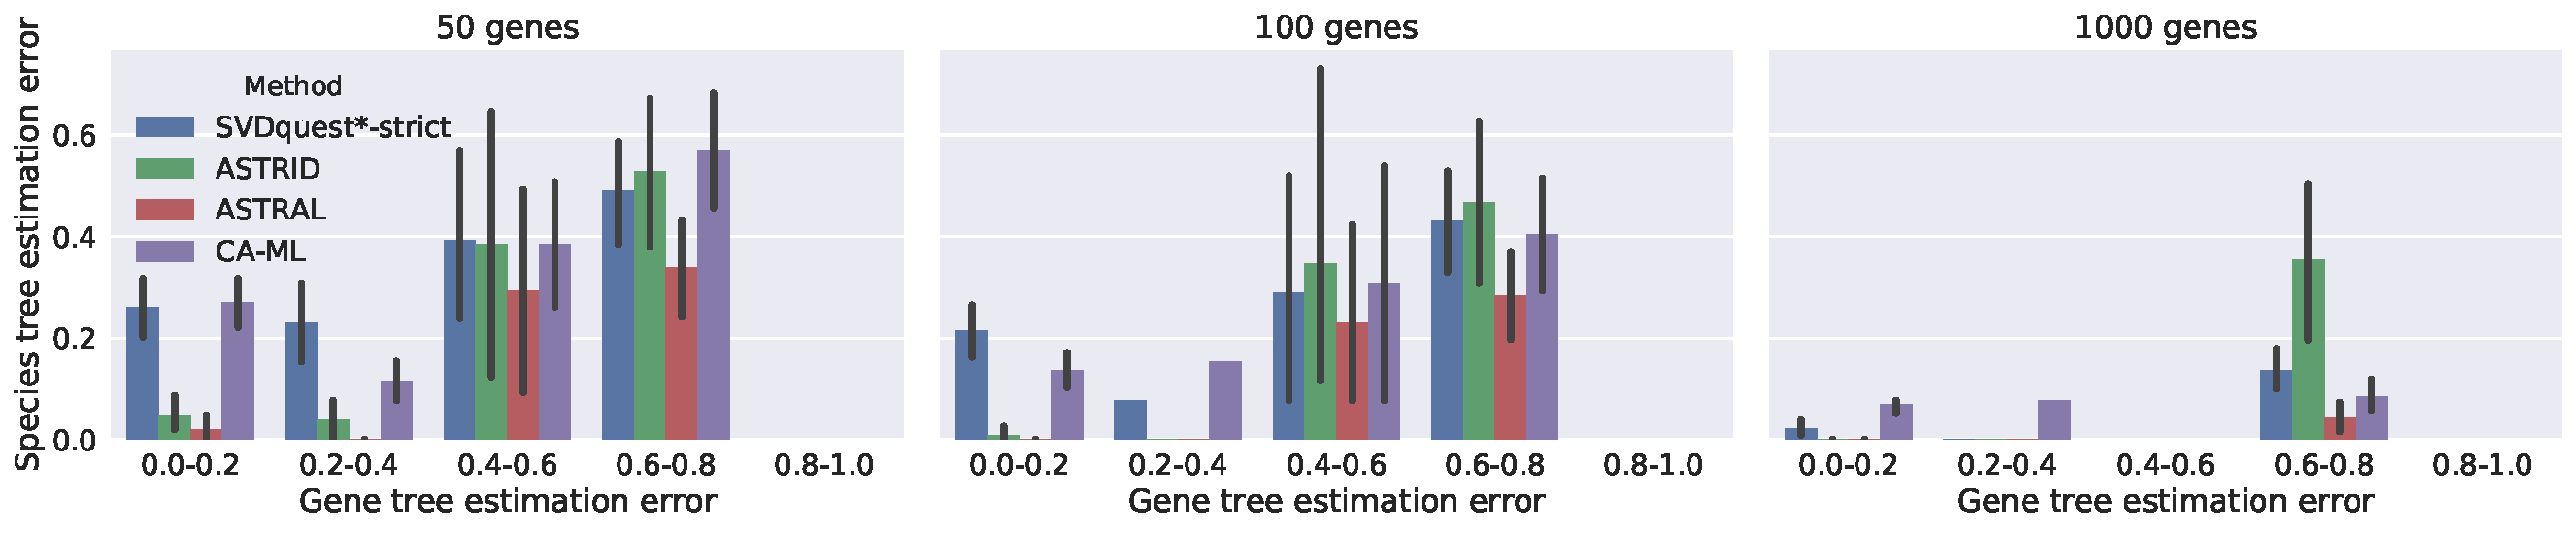
\includegraphics[width=\textwidth]{svdquest-figs/concat_rfdists_15tax.pdf}
\caption[Species tree topological error rates for 15-taxon simulated data as a function of gene tree estimation error]{Species tree topological  error rates (maximum possible is 1.0) 
  for 15-taxon simulated data (AD=82\%), as a
    function of gene tree estimation error (maximum possible is 1.0). Error bars show standard
    error over 10 replicates.
      }
\label{svdquest::fig:exp3_15}\end{figure}


\begin{figure}
  \centering
  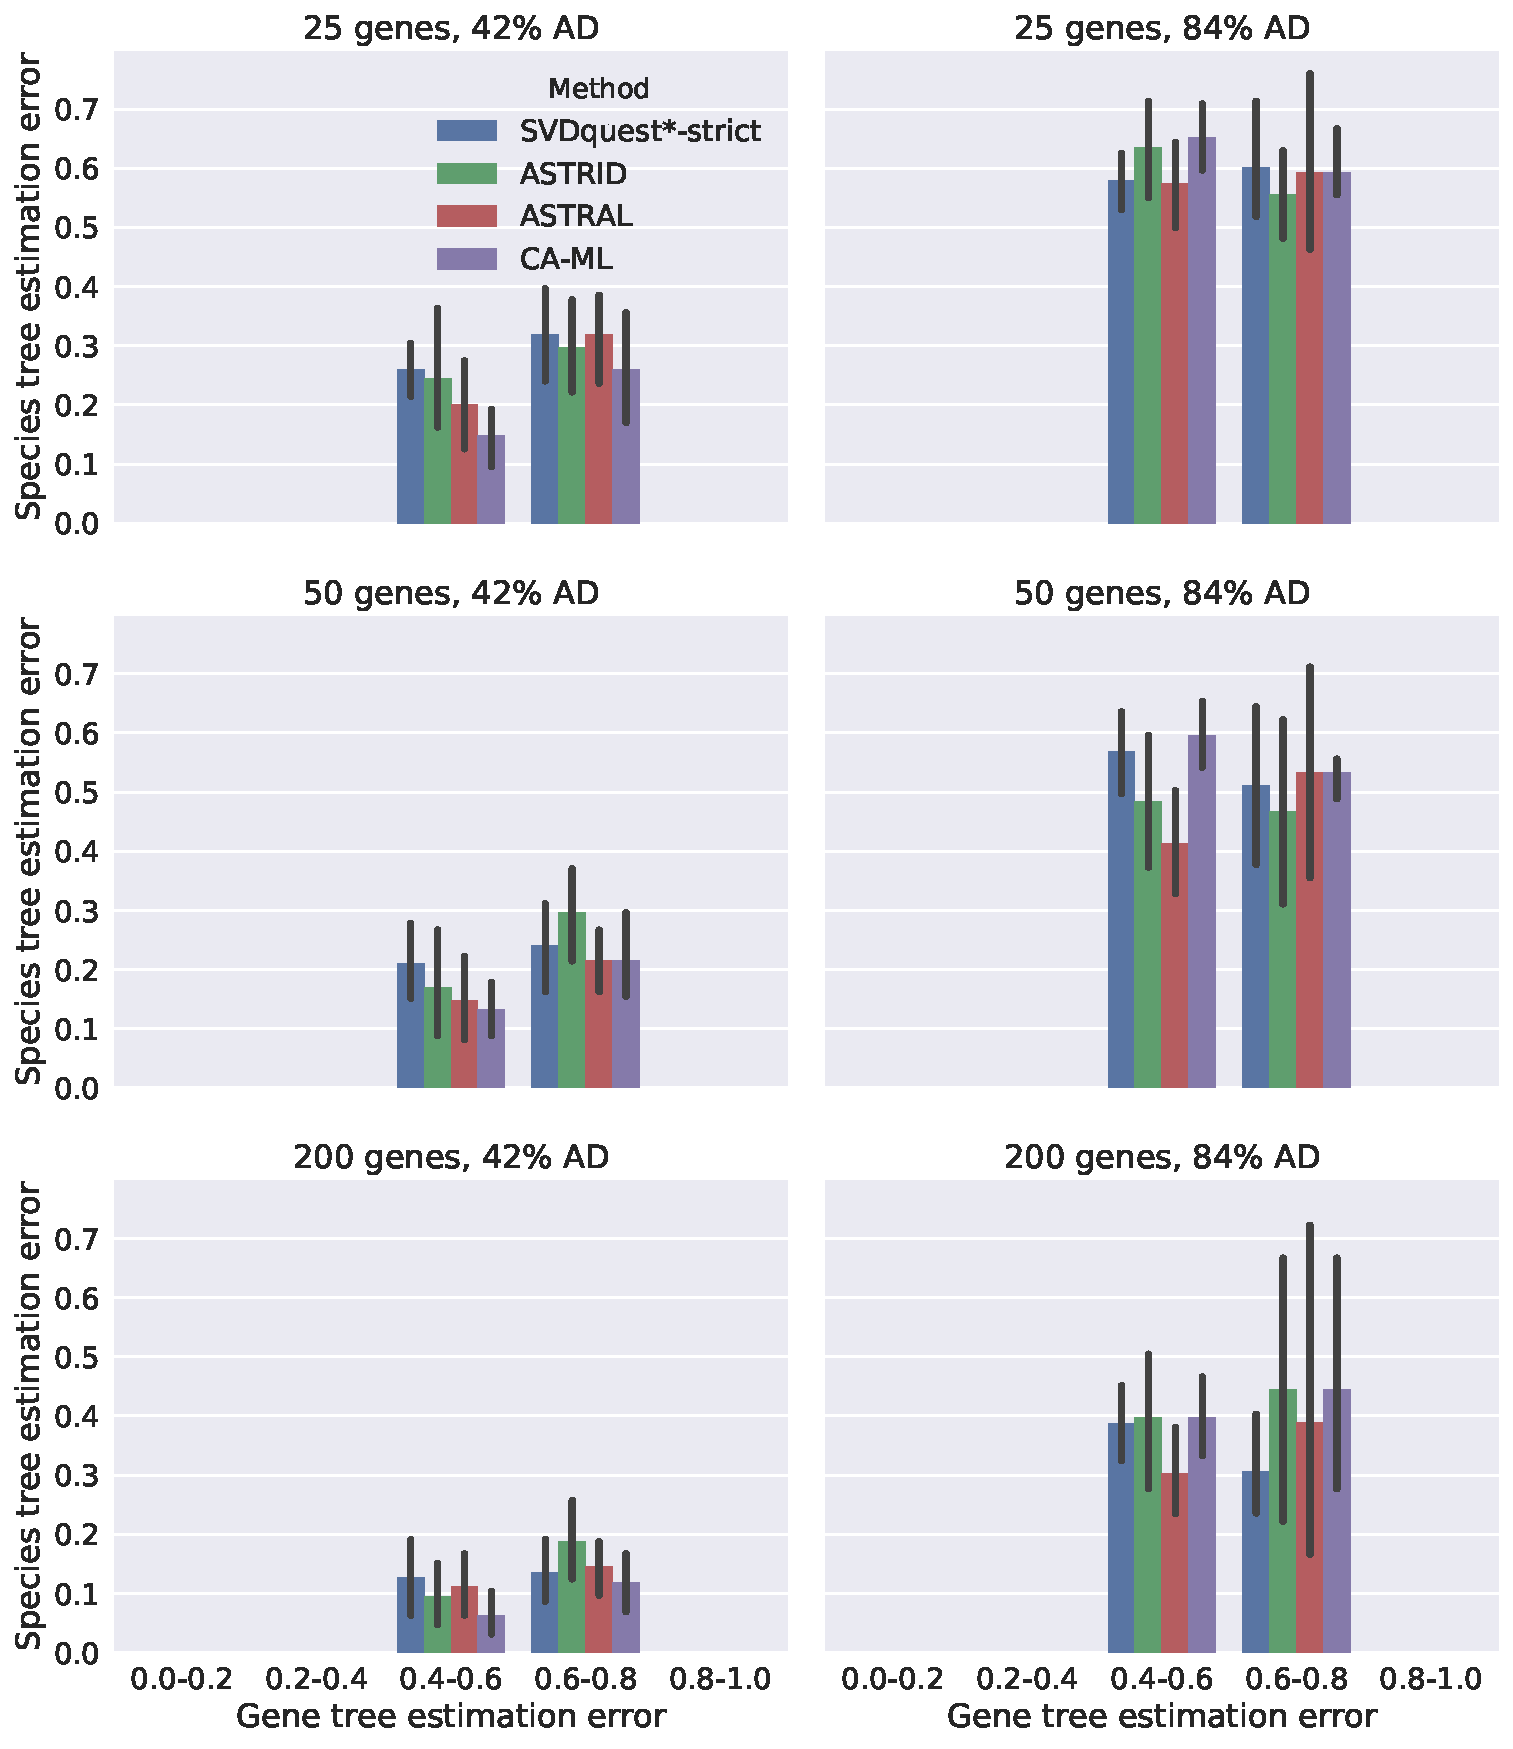
\includegraphics[width=0.8\textwidth]{svdquest-figs/concat_rfdists_10tax.pdf}
  \caption[Species tree topological error rates for 10-taxon simulated data as a function of gene tree estimation error]{Species tree topological error rates (maximum possible is 1.0) for 10-taxon simulated data, as a
    function of gene tree estimation error (maximum possible is 1.0). Error bars show standard
    error over 10 replicates.
    }
\label{svdquest::fig:exp3_10}\end{figure}


\clearpage
\section{Discussion}

\paragraph{MQSST scores. }
By design, it is impossible for SVDquest* to produce a tree with a
worse MQSST score than SVDquartets+PAUP*. Hence, the question is how much better
SVDquest* is than SVDquartets+PAUP* at finding good MQSST scores, and how the
different model conditions affect the frequency with which
SVDquest* improves on SVDquartets+PAUP*.


Our data show that SVDquest* often finds better scores than SVDquartets+PAUP*, but
the frequency of this improvement  depends on the model conditions, and is clearly related to the difficulty
of the MQSST problem instance. 
Obviously, if
SVDquartets+PAUP* finds an optimal solution,  there is no better solution
for SVDquest* to find.
More generally,  conditions that make it easy to find near-optimal MQSST using PAUP*'s heuristic search
strategies will make it difficult for SVDquest* to do better than SVDquartets+PAUP*. 
ILS levels and number of genes both impact the relative performance, with an increasing advantage to
SVDquest* over SVDquartets+PAUP* as ILS level increases or as the number of genes decreases. 
Both these trends are consistent with the hypothesis that easy conditions tend to reduce the advantage of SVDquest* over SVDquartets+PAUP* at
finding good solutions to MQSST.
The impact of GTEE is more complicated. 
Below about 30\% GTEE, SVDquartets+PAUP*
often finds a good MQSST score, so there is less room for SVDquest* to
find an improvement.  
Above approximately 80\% GTEE,
 SVDquartets+PAUP* might not find a good solution, but the gene trees
have so much error that the constraint set computed by SVDquest* does
not include parts of the solution space where better trees can be
found.
However, under other conditions (i.e., 
when GTEE
is neither extremely low or extremely high),
 SVDquest* tends to produce better MQSST scores than SVDquartets+PAUP*.



These observations provide insights into the impact of
GTEE on SVDquest*.
It is well known that summary methods, such as
ASTRAL and ASTRID,
directly rely on estimated gene trees, and
compute  species trees 
based on summary statistics on the gene trees - quartet
distributions or average internode distances.  In contrast, gene tree
estimation error only impacts how SVDquest* constrains the search
space, and does not impact the criterion scores of any trees it can
examine.  Furthermore, the only real problem with using poorly
estimated gene trees occurs when all the estimated gene trees are poor
-- because then the bipartitions of the true species tree may not end
up in the constraint set. 
Adding bipartitions from poor gene trees to  the constraint set
 expands the search space
and hence increases the running time, but will never reduce the
criterion score produced by SVDquest*.  
This suggests a general
strategy of adding estimated species trees to the constraint set, even those that are not
likely to be highly accurate; these expand the search space for
SVDquest*, and are useful as long as they have a positive probability of containing a
bipartition from a higher-scoring tree.



\paragraph{Species tree accuracy. }


A comparison between SVDquartets+PAUP* and SVDquest*-strict with respect to topological accuracy reveals that
generally the differences are small, but that when the trees are different there is usually an improvement obtained
by using SVDquest*-strict. 
The difference in accuracy is often small, but can be large (i.e., up to 10-15\% in normalized RF). 
Hence, SVDquest*-strict provides an advantage (although slight) over SVDquartets+PAUP* in terms of species tree topology estimation.

The relative performance of ASTRAL and ASTRID in our study generally favored ASTRAL,
in the
sense that although the two methods were often very close in accuracy (and sometimes
had identical accuracy), ASTRID was more impacted by GTEE than ASTRAL, and so was
less accurate for the conditions with very short loci. 
 
Both summary methods had very good accuracy -- outperforming the other methods --
when GTEE was sufficiently low and ILS was sufficiently high.
However, 
CA-ML had the best accuracy
under sufficiently low ILS levels, and even had  the best accuracy
under high ILS levels when GTEE was
sufficiently high. 
SVDquest*-strict was less accurate than ASTRAL and ASTRID when GTEE was sufficiently low, but
was  as accurate as ASTRID and ASTRAL, and sometimes more accurate, when 
GTEE was very high.

Finally, although CA-ML typically dominated SVDquest*-strict, there
were  a few  10-taxon model conditions where SVDquest*-strict improved on the accuracy of CA-ML. 
Specifically, on the 10-taxon model conditions with high ILS (84\% AD), high GTEE, and at least 50 
genes, SVDquest*-strict was slightly more accurate than CA-ML.
%Figure 12




\paragraph{Comparison to prior studies. }


Several other studies  (surveyed in \cite{MolloyWarnow2017}) have compared coalescent-based methods  and CA-ML under various simulated model conditions.
These studies made the same general observations about the relative performance between the summary methods and CA-ML. 
Two prior studies \cite{Chou2015,MolloyWarnow2017} have  compared SVDquartets+PAUP*  to  other methods, including ASTRAL,  NJst, ASTRID, and CA-ML;
although SVDquartets+PAUP* sometimes improved over the summary methods when GTEE was sufficiently high, it was only
rarely more accurate than CA-ML. 
Although we report results for SVDquest*-strict (which directly improves on SVDquartets+PAUP*  for optimizing
MQSST trees), our  findings are also consistent with these general trends.

It is not clear what factors influence the relative accuracy of SVDquartets-based methods and CA-ML, although these studies as a whole
suggest that when ILS is low enough, then CA-ML should be more accurate than SVDquest*-strict and SVDquartets+PAUP*.
The total number of sites also seems to influence the relative performance, so that under high enough ILS and a large enough number of
sites, SVDquartets-based methods may have an advantage over CA-ML.
However, in our studies, when there was an advantage, it was small.


 Experiment 3 suggests that species trees based on supergene trees
(instead of on trees computed on c-genes)
 can sometimes improve the accuracy of species trees computed using
 SVDquest*-strict, as well as ASTRAL and ASTRID.
 The improvement for ASTRAL and ASTRID is consistent with
a similar study (but applied to different summary methods) where supergenes are also based on random collections of genes \cite{bayzid2013naive}; furthermore, 
\cite{LanierKnowles2012}  also observed that coalescent-based summary
methods were generally robust to recombination within loci.
The  improvement is perhaps surprising, since current
theoretical justifications for using summary methods require that the
loci be recombination-free. Furthermore, \cite{SpringerGatesy2016} argue
that recombination-free loci may be extremely short (as few as 12 base
pairs), and point out that on this basis the theoretical justification
of summary methods is flawed.  This concern is justified. However,
from an empirical standpoint the results in these experiments suggest
that failure to break loci into recombination-free regions may not be
a substantial problem - and may even lead to improvements in some
(but not all)
cases.

 
\paragraph{Running time considerations. }


Our study also examined running time, and showed that SVDquest*-strict was reasonably fast. However, 
SVDquest*  needs ASTRAL and SVDquartets+PAUP* to compute the constraint set, and so 
is necessarily more computationally intensive than both SVDquartets+PAUP* and ASTRAL.
By far the dominant part of the running time for SVDquest*-strict  is the gene tree estimation part,  but this can be parallelized (i.e., each gene tree
can be calculated independently of the others).
In particular, it is feasible to run 
SVDquest*-strict on any dataset on which the full set of quartet trees can be computed using SVDquartets, which  is also easily parallelized.



\paragraph{Future Work}

This study suggests multiple directions  for future research.
We used the default setting within PAUP* and 
we computed quartet trees for every four leaves; these choices are  supposed  to maximize the accuracy of SVDquartets+PAUP*, 
but it is possible that some other
way of combining quartet trees within PAUP* would result in topologically more accurate trees.
Similarly, quartet tree amalgamation is a basic algorithmic problem, and
SVDquartets+PAUP* could be improved through the use of new quartet amalgamation methods.
In addition, a branch-swapping heuristic could be developed that begins with the SVDquest* tree and searches for
better solutions to MQSST; thus, 
 SVDquartets+PAUP* can also be improved by incorporating SVDquest* as a starting tree. 
Furthermore, the basic strategy within SVDquest* of using other species tree methods to add bipartitions to the constraint set
enables SVDquest to remain useful, even as PAUP* improves through the use of new quartet amalgamation heuristics.
 
Another interesting direction would be to modify the optimization problem that we solve.
Thus, in the MQSST problem, there is exactly one tree on every four species, and  
each of these quartet trees has unit weight. 
A weighted version of MQSST would be very interesting to examine, where
instead of taking the best topology for each four taxa, the three
possible topologies are weighted based on their SVD scores
or on the statistical support for
the quartet tree \cite{GaitherKubatko2016}.

 
 SVDquest*-strict could also be compared to PoMo \cite{pomo} and its improved version revPoMo \cite{revPomo}, which
estimate species trees from multi-locus datasets under a model of site evolution that allows each node in the tree to be polymorphic. While these methods have not been shown to be statistically consistent under the MSC, they have shown very good accuracy on simulated data, even when gene tree heterogeneity due to ILS is present, and so may provide
excellent accuracy in practice.
   
The accuracy of SVDquartets for computing quartet trees on biological datasets is not well understood, and this also presents multiple opportunities for
future research.
For example,  this study examined the use of SVDquest* with multi-locus datasets, and  assumed that gene trees can be
computed on each of the loci. 
However, the basic algorithmic strategy  in SVDquest can be used with SNP data as well, as we now describe.
When the number of species is small enough (i.e., at most 20),  then SVDquest could be used in its unconstrained mode:  quartet trees can be computed using SVDquartets, and then a species tree 
optimizing the MQSST score can be found using the dynamic programming algorithm in SVDquest.
For datasets with larger numbers of species, the constrained version can be used in several ways.
For example,  the constraint set can be initialized to the bipartitions in the SVDquartets+PAUP* tree, and then enlarged using standard CA-ML analyses, PoMo and revPomo (as described
earlier), trees computed on bootstrap replicates, or other techniques.   
Similarly, our study examined SVDquest* on supergene datasets (formed by randomly concatenating c-genes) and showed good accuracy, but true recombination will produce patterns that are somewhat different, and the impact of
recombination on SVDquest* and summary methods needs to be explored.

  Another limitation of our study is that the simulations we performed evolved sequences only with substitutions (i.e., no insertions
 and deletions), and so alignment estimation was not necessary;  yet alignment
 error is quite common in practice, especially when the datasets span 
 large evolutionary timescales. 
 Although alignment error also increases gene tree estimation error, several studies have
shown that accurate gene trees can be computed even in the presence of
some alignment error \cite{sate2009}, so that it is possible that SVDquest* and other
site-based methods could be more negatively impacted than summary methods.
Hence, the impact of alignment error is an important aspect to consider.
 If alignment error negatively impacts SVDquartets, it may be that approaches that select sites within alignments to use within SVDquartets will be helpful.
  
Finally, although SVDquest*-strict is fast enough to be used on 
whole genome datasets with moderately large numbers of species, we only tested SVDquest*-strict under conditions where
all quartet trees could be computed.
Therefore, when the number of species is large enough (i.e., 200 or more), then this becomes computationally infeasible.
For this reason, when the number of species is too large, PAUP* uses random sampling on the quartets, uses SVDquartets to compute quartet trees, and then
combines these quartet trees using its quartet amalgamation heuristics. 
In its current implementation, 
SVDquest cannot be used with such inputs, but 
the dynamic programming algorithm  in SVDquest  can be used with any way of weighting quartet trees, and so could be used with sparsely sampled quartet trees by assigning
equal weights to all three quartet trees on any unsampled quartet. 
However, sparse sampling of quartet trees for use with quartet amalgamation methods has been shown to have reduced
accuracy compared to analyses that use all the quartet trees \cite{Swenson2011}, suggesting that when the number of species makes SVDquest* inapplicable, 
summary methods or concatenation may be a better choice than SVDquartets-based approaches.
Thus, the best modifications to SVDquest* to enable it to be used to good advantage on datasets with large numbers of species will
require some investigation. 
 



\section{Summary}


We presented SVDquest*, a site-based
method for species tree estimation.
Like the implementation within PAUP* (which we
refer to as SVDquartets+PAUP*), SVDquest* operates by
computing quartet trees using SVDquartets, and
then seeks a species tree with 
the largest  MQSST  score.  Unlike
SVDquartets+PAUP*, which uses a heuristic
search through treespace, 
SVDquest* uses an exact algorithm for this optimization
problem, and achieves polynomial time by constraining the search
space using a set of bipartitions on the species set that it
computes from the input. 
By design, SVDquest* is
guaranteed to obtain a score that is at least as  large
as the score 
produced using SVDquartets+PAUP*. 
In practice, SVDquest* typically finds
trees with better MQSST scores than SVDquartets+PAUP*, especially on datasets with
higher levels of  gene tree
estimation error and lower numbers of genes. 




Our study evaluated SVDquest*-strict in comparison to two summary methods (ASTRAL and ASTRID), 
SVDquartets+PAUP*, and CA-ML under a wide range of ILS levels, numbers of species, and numbers of genes.
Although our study was limited to conditions with at most 1000 genes and 50 species, we observed
several significant and interesting trends. 
While ASTRAL and ASTRID can be more accurate than
SVDquest*-strict when GTEE is low, 
SVDquest*-strict is typically more accurate than these summary methods when GTEE is high, as GTEE impacts
summary methods directly, introducing error into the summary statistics they use to construct species trees.
CA-ML is surprisingly accurate, and more accurate than
the summary methods under conditions with high GTEE (even when ILS is high);
interestingly,  we also observed that sometimes SVDquest*-strict improves on CA-ML.
Thus, the relative accuracy between these methods depends on the model condition, and in particular on the ILS 
and GTEE levels, but SVDquest*-strict provides advantages over the other coalescent-based methods under 
several biologically realistic conditions. 

This study also shows  that SVDquest*-strict is fast enough to use on  genome-scale biological 
datasets. 
SVDquest*-strict includes calls to  both ASTRAL  and SVDquartets+PAUP*, and is otherwise very fast; 
hence, any dataset on which both of these methods can be run can be analyzed by SVDquest*-strict.
Furthermore, a comparison of running times between these methods and concatenation  suggests that
for large enough datasets, concatenation analyses are likely to become computationally extremely expensive. 
For example,  a concatenated maximum
likelihood analysis of the 48-species avian phylogenomics dataset with 14,446 loci took more than 200 CPU years \cite{jarvis2014whole}, while
an analysis using the new implementation of ASTRAL took only 32 hours after the gene trees were computed \cite{astral3}.
The calculation of 14,446 ML gene trees is expensive, but completes in well under a month (and is very fast if
parallelized) \cite{jarvis2014whole}.
Hence, summary methods are generally computationally much more feasible than concatenation analyses for large
datasets, which means that SVDquest*-strict is a computationally feasible approach for many  genome-scale datasets.
 
This study adds to the current literature evaluating site-based approaches to species tree estimation.
Although we did not find that SVDquest*-strict improved on the competing coalescent-based approaches under all conditions,
our study shows that SVDquest*-strict can provide improved accuracy under  some conditions with high GTEE.
This trend suggests the potential for
SVDquest*-strict to be particularly beneficial for genome-scale datasets,  where GTEE is likely to be high as a result of
either ILS or variable rates of evolution across the genome. 
In addition, SVDquest*-strict had very good accuracy on supergene datasets, suggesting it may be robust to failure to detect recombination events.
Finally, the relative performance between SVDquest*-strict (and other methods based
on SVDquartets),  summary methods, and CA-ML might well depend on the number of
loci, so that SVDquest*-strict (or other methods based on SVDquartets) could become the method of choice when the number of loci and ILS level are both very large.
 

\begin{figure}
  \centering
  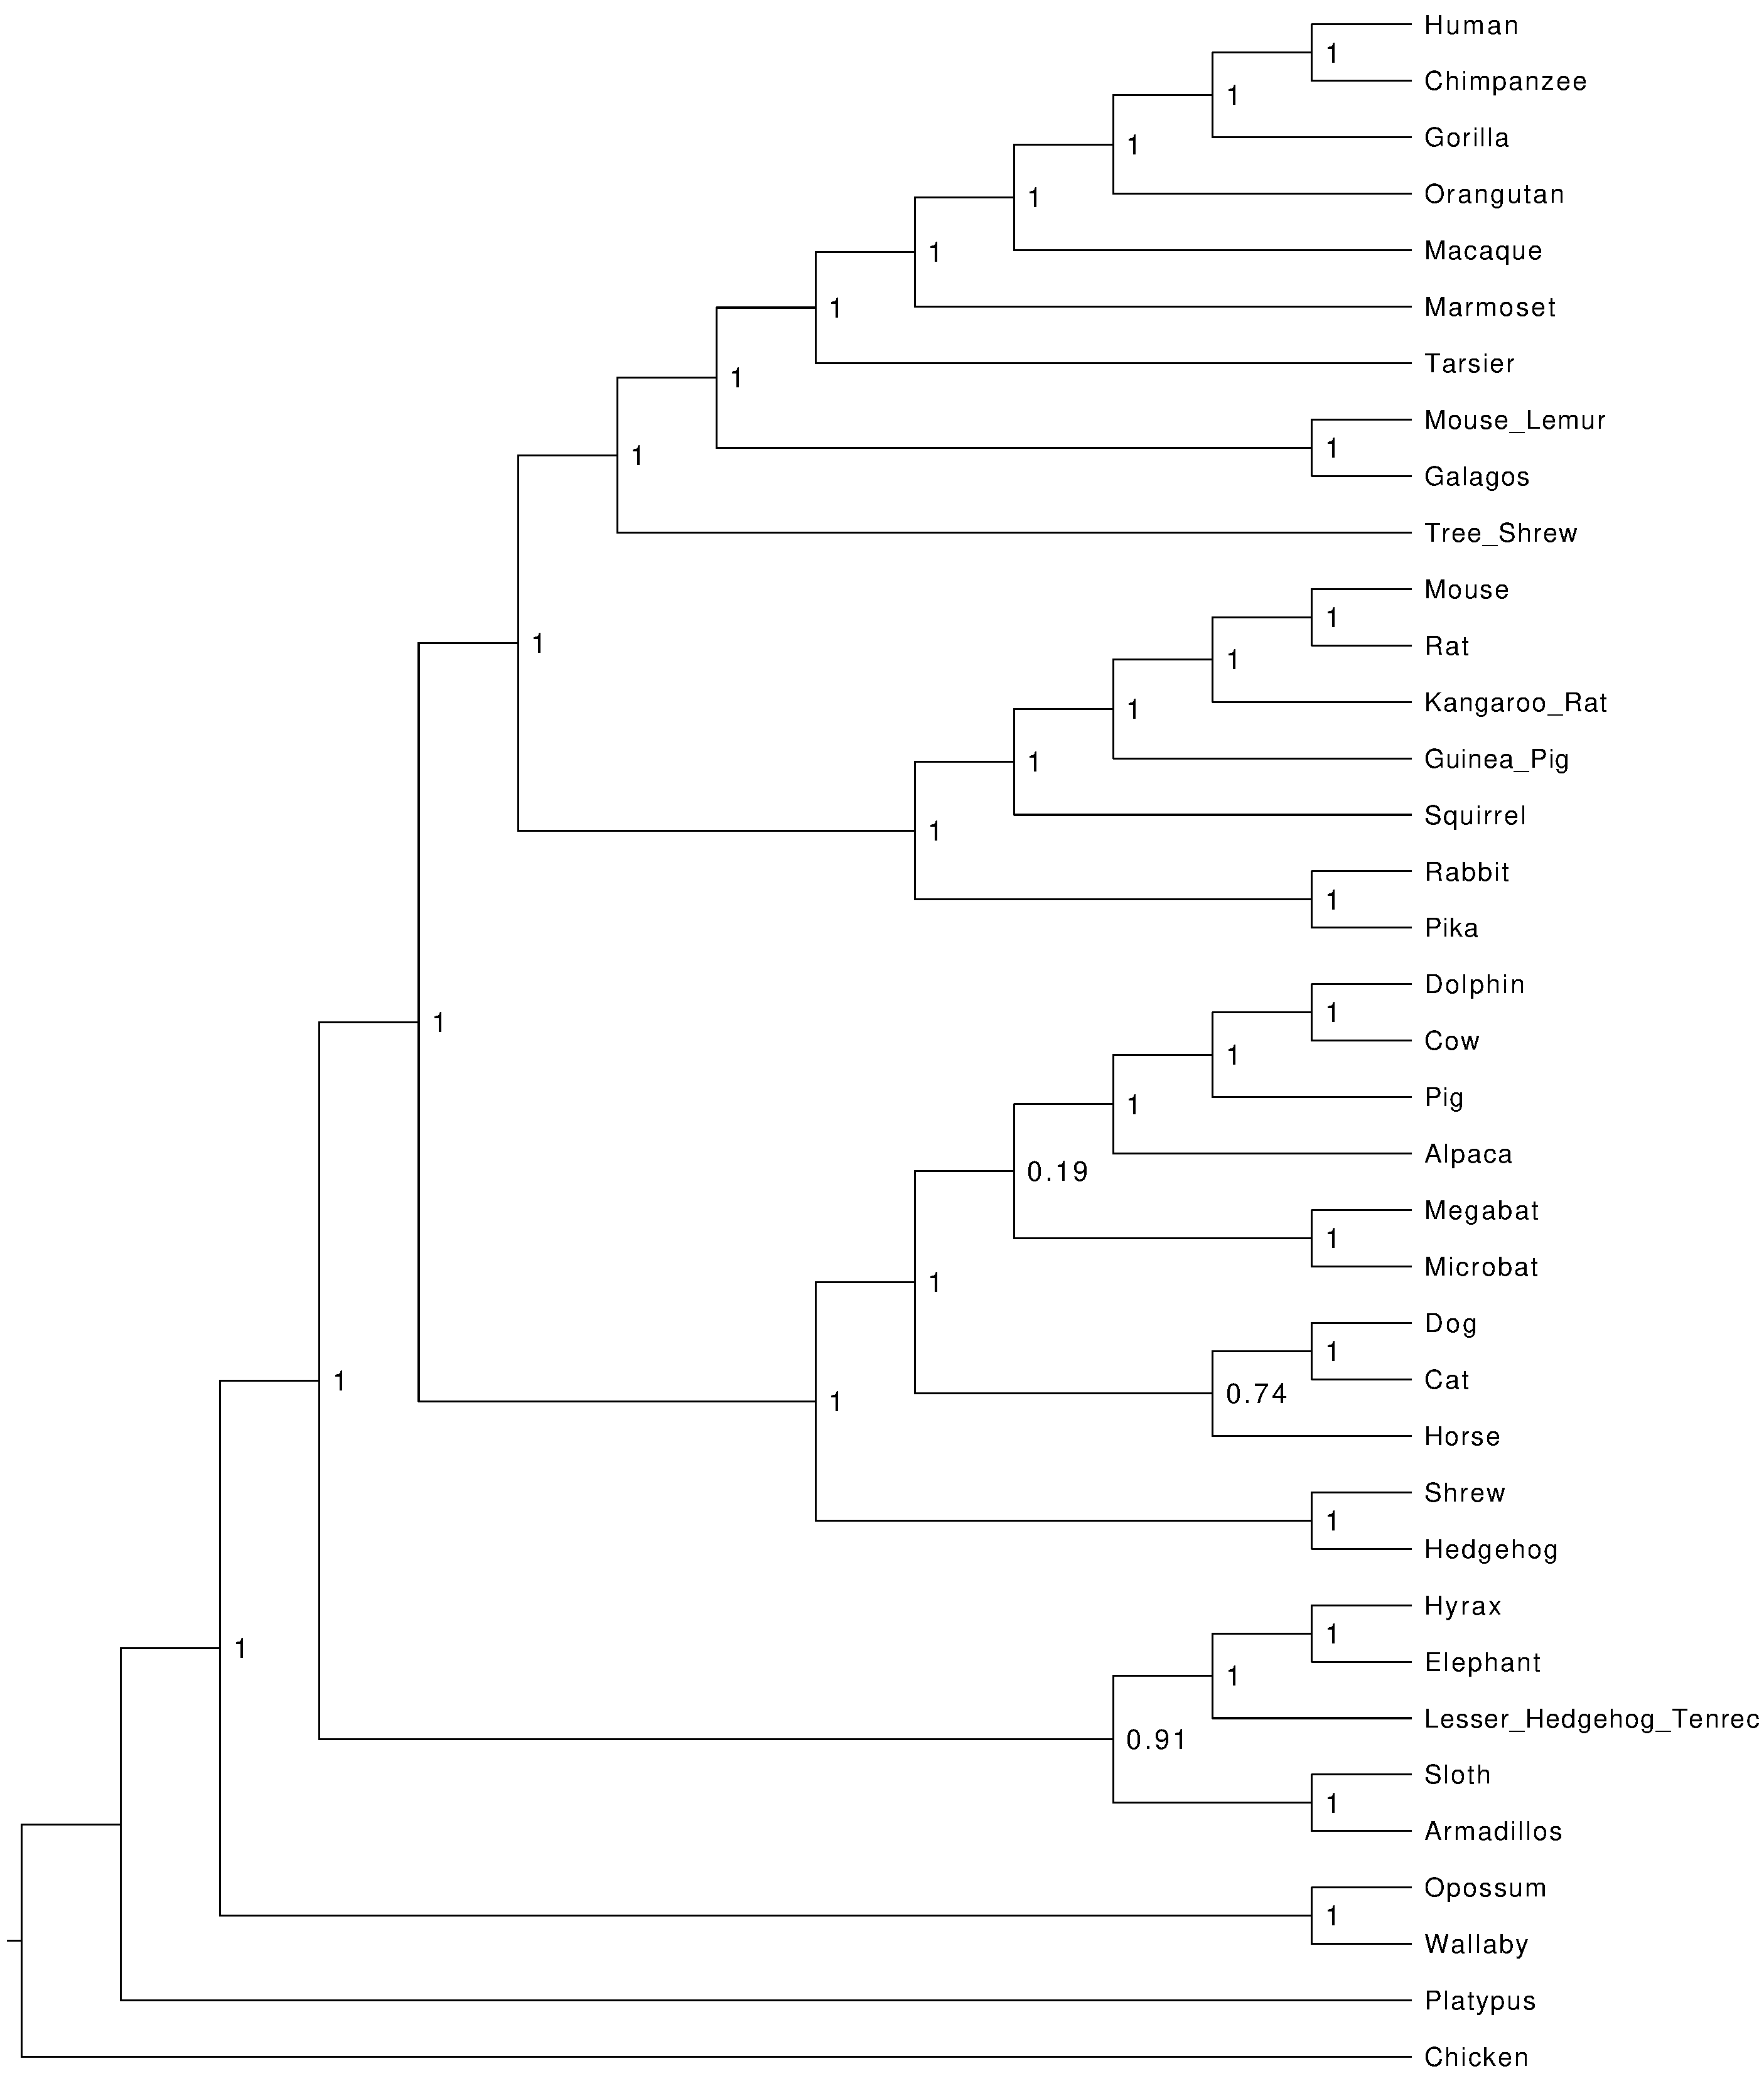
\includegraphics[width=\textwidth]{svdquest-figs/fully-parametric-mammalian.pdf}
  \caption{Mammalian SVDquest* tree with branch support, computed using a modified non-parametric bootstrapping approach, from 100 bootstrap replicates.}
  \label{svdquest::fig:mammalian-svdquestplus}
\end{figure}
